\documentclass[a4paper,12pt,english]{report}
\usepackage[T1]{fontenc}
\usepackage[utf8]{inputenc}
\usepackage{lmodern}  
\usepackage{textcomp}
\usepackage{booktabs}
\usepackage{listings}
\usepackage{xcolor}

\lstdefinelanguage{json}{
	basicstyle=\ttfamily\small,
	showstringspaces=false,
	breaklines=true,
	frame=single,
	backgroundcolor=\color{gray!5},
	string=[s]{"}{"},
	stringstyle=\color{blue},
	comment=[l]{:},
	commentstyle=\color{black},
}

\usepackage[english]{babel}
\renewcommand{\contentsname}{Table of Contents}
\usepackage{geometry}
\usepackage[english]{minitoc}
\usepackage[dvipsnames, table]{xcolor}
\usepackage{amsmath, amssymb, amsthm}
\usepackage{cases}
\newtheorem{theorem}{Theorem}
\newtheorem{definition}{Definition}
\newtheorem{example}{Example}
\newtheorem{proposition}{Proposition}
\newtheorem{lemma}{Lemma}
\usepackage{upgreek}
\newtheorem{observation}{Observation}
\usepackage{enumitem}
\usepackage{graphicx}
\graphicspath{ {./images/} }
\usepackage{lipsum}
\usepackage{lscape}
\usepackage{rotating}
\usepackage[linesnumbered,ruled,vlined]{algorithm2e}
\usepackage[unicode, colorlinks, linkcolor=Blue, hypertexnames=false]{hyperref}
\usepackage{fancyhdr}
\usepackage{amssymb}
\usepackage[nohyperlinks]{acronym}  
\usepackage{pgfplots}
\usepackage{adjustbox}
\usepackage{array,multirow,makecell}
\usepackage{tabularx}
\newtheorem{algo}{Algorithme}
\pagestyle{fancy}
\pgfplotsset{compat=1.18}
\usepackage{ctable} 
\usepackage{float}
\usepackage{url}
\usepackage{blindtext, color}
\usepackage{titlesec}
\titleformat*{\subsubsection}{\itshape}
\renewcommand{\thesubsubsection}{\Alph{subsubsection}.}
\definecolor{gray75}{gray}{0.75}
\newcommand{\hsp}{\hspace{20pt}}
\titleformat{\chapter}[block]{\Huge\bfseries}{\thechapter\hsp\textcolor{gray75}{|}\hsp}{0pt}{\Huge\bfseries}
\setcellgapes{1pt}
\makegapedcells
\newcolumntype{R}[1]{>{\raggedleft\arraybackslash }b{#1}}
\newcolumntype{L}[1]{>{\raggedright\arraybackslash }b{#1}}
\newcolumntype{C}[1]{>{\centering\arraybackslash }b{#1}}
\setcounter{secnumdepth}{3}
\setcounter{tocdepth}{3}
\fancyhf{}
\renewcommand{\chaptermark}[1]{\markboth{#1}{}} 
\renewcommand{\sectionmark}[1]{\markright{\thesection\ #1}}
\fancyfoot[C]{\textbf{\thepage}}
\fancyhead[L]{\textsl{\rightmark}}
\setlength{\headheight}{14.5pt}
\headsep = 25pt
\headwidth=16.50cm
\renewcommand{\headrulewidth}{0.1pt} 
\geometry{top=2.5cm, bottom=2.5cm, left=2.5cm, right=2cm}
\renewcommand{\baselinestretch}{1.15}
\newcommand{\tolstrut}{%
  \vrule height\dimexpr\fontcharht\font`\A+.1ex\relax width 0pt\relax
}
\DeclareRobustCommand{\textoverline}[1]{%
  \ensuremath{\overline{\mbox{\tolstrut#1}}}%
}
\usepackage[nottoc]{tocbibind}
\makeatletter
\newcounter{subsubsubsection}[subsubsection]
\renewcommand\thesubsubsubsection{\thesubsubsection .\@alph\c@subsubsubsection}
\newcommand\subsubsubsection{\@startsection{subsubsubsection}{4}{\z@}%
                                     {-3.25ex\@plus -1ex \@minus -.2ex}%
                                     {1.5ex \@plus .2ex}%
                                     {\normalfont\normalsize\bfseries}}
\renewcommand\paragraph{\@startsection{paragraph}{5}{\z@}%
                                    {3.25ex \@plus1ex \@minus.2ex}%
                                    {-1em}%
                                    {\normalfont\normalsize\bfseries}}
\renewcommand\subparagraph{\@startsection{subparagraph}{6}{\parindent}%
                                       {3.25ex \@plus1ex \@minus .2ex}%
                                       {-1em}%
                                      {\normalfont\normalsize\bfseries}}
\newcommand*\l@subsubsubsection{\@dottedtocline{4}{8.0em}{4.1em}}
\renewcommand*\l@paragraph{\@dottedtocline{5}{10em}{5em}}
\renewcommand*\l@subparagraph{\@dottedtocline{6}{12em}{6em}}
\newcommand*{\subsubsubsectionmark}[1]{}
\makeatother
% Cover page extra packages
\usepackage{tikz}
\usepackage{setspace}
% Bibliography style is set below near \bibliography call

%--------------------------------------------------------------
\begin{document}

%--------------------------------------------------------------
% COVER PAGE — Official Horizon University Template
%--------------------------------------------------------------
\begin{titlepage}
    \begin{center}
        % Header: University name left, Ministry right
        \begin{minipage}{0.45\textwidth}
            \centering
            Private University\\
            Horizon School of Digital\\
            Technologies\\
        \end{minipage}
        \hfill
        \begin{minipage}{0.45\textwidth}
            \centering
            Republic of Tunisia\\
            Ministry of Higher Education\\
            and Scientific Research
        \end{minipage}
        \vspace{1cm}

        % Horizon Logo
        
\includegraphics[width=0.6\textwidth]{logo_horizon.png}

        \vspace{0.7cm}

        % Background image block + main cover content
        \begin{tikzpicture}[remember picture, overlay]
            \node[opacity=0.5, inner sep=0pt, anchor=center] at (current page.center) {
                
\includegraphics[width=\paperwidth]{bg.png}
            };
        \end{tikzpicture}

        {\Large \textbf{End Of Studies Project Report}} \\
        \vspace{0.5cm}
        {Presented in order to obtain the National \textbf{Bachelor's Degree} in} \\
        \vspace{0.3cm}
        {\large \textbf{Computer Science}} \\
        \vspace{0.2cm}
        {Major: {\large \textbf{Software Engineering and Information Systems}}}

        \vspace{1.5cm}

        % Project Title Box
        \begin{minipage}{0.85\textwidth}
            \centering
            \rule{\linewidth}{0.5pt} \\
            \vspace{0.3cm}
            \large \textbf{VisionTest-AI: An Intelligent Agent for Autonomous Functional Testing using NLP and Computer Vision} \\
            \vspace{0.3cm}
            \rule{\linewidth}{0.5pt}
        \end{minipage}

        \vspace{1cm}

        % Author
        {\large By: \textbf{Nour El Karia}}

        \vfill

        % Jury Table
        \vspace{0.3cm}
        {Defended on \quad / \quad / 2026 \quad in front of the jury composed of:} \\
        \vspace{0.8cm}
        \begin{flushleft}
            \begin{tabular}{ll}
                Mr./Mme : ............................................\hspace{3.4cm} President \\
                Mr./Mme : ............................................\hspace{3.4cm} Reviewer \\
                Mme Noura Aboudi \hspace{4.15cm} Academic Supervisor \\
                M. Baha Rahmouni \hspace{4.45cm} Professional Supervisor \\
            \end{tabular}
        \end{flushleft}

        \vspace{0.5cm}
        % Company logo (ADDINN / Orange internship company)
        
\includegraphics[width=2.5cm]{Addine_logo.png}

        \vspace{0.4cm}
        \begin{center}
            Réf : .......... \\
            \vspace{0.6cm}
            \rule{4cm}{0.5pt} \quad Année Universitaire : 2025 -- 2026 \quad \rule{4.5cm}{0.5pt}
        \end{center}

    \end{center}
\end{titlepage}
%--------------------------------------------------------------
% REST OF DOCUMENT
%----------------------------------------------------------------
\setcounter{minitocdepth}{2}
\dominitoc
\titlespacing*{\chapter}{0pt}{50pt}{40pt}
\pagenumbering{roman}
\chapter*{Dedication}
\addcontentsline{toc}{chapter}{Dedication}

\vspace*{2cm}

\begin{center}
	\textit{I dedicate this work...}
	
	\vspace{1cm}
	
	\textit{To \textbf{God Almighty}, for His infinite grace and for lighting my path.}
	
	\vspace{0.6cm}
	
	\textit{To my \textbf{Parents}, my first teachers and greatest supporters. Your love and sacrifices are the foundation of my success.}
	
	\vspace{0.6cm}
	
	\textit{To my \textbf{Sisters and Brother}, for your encouragement and for always believing in me.}
	
	\vspace{0.6cm}
	
	\textit{To my dear friends Thank you for the shared journey, the motivation, and the unforgettable memories.}
	
	\vspace{0.6cm}
	
	\textit{To the \textbf{Horizon School of Digital Technologies}, for the academic excellence that shaped my future.}
\end{center}


\mtcaddchapter
\chapter*{Acknowledgments}
\addcontentsline{toc}{chapter}{Acknowledgments}

\vspace{1cm}

First and foremost, I wish to express my gratitude to the Almighty \textbf{God} for providing me with the strength and perseverance required to complete this work.

I would like to acknowledge my professional supervisors at \textbf{ADDINN Group}, \textbf{M. Mohamed Essid} and \textbf{M. Baha Rahmouni}, for their presence and for the opportunity to conduct my final year project within the company's Data/AI department.

I am especially honored to express my deepest and most sincere gratitude to my academic supervisor, \textbf{Mme Noura Aboudi}. I am profoundly grateful for her invaluable guidance, her constant availability, and the scientific rigor she provided throughout this journey. Her unwavering support and encouragement were essential in overcoming the technical challenges of this project and ensuring its academic success.

I also wish to extend my appreciation to the \textbf{Members of the Jury} for their time and effort in evaluating this work, as well as to the staff of the \textbf{Horizon School of Digital Technologies} for the education I have received over the years.

Finally, I thank all my colleagues at \textbf{ADDINN Group} for the professional environment provided during my internship.

\vspace{1cm}

\begin{flushright}
	\textbf{Nour El Karia}
\end{flushright}
\mtcaddchapter
\chapter*{Abstract}
\addcontentsline{toc}{chapter}{Abstract}
\hrule
\vspace{1.2cm}

Functional test automation is an important part of modern software quality assurance, especially in Agile and DevOps environments where applications change frequently. However, automated tests often remain fragile because they depend on technical selectors, DOM structure, and manually written scripts. A small change in the user interface can break a test even when the business behavior of the application is still correct.

This end-of-studies project, carried out within \textbf{ADDINN Group}, presents \textbf{VisionTest-AI}, an intelligent functional testing agent designed to reduce this fragility. The system starts from business-readable Gherkin scenarios and transforms them into executable browser actions. It combines Natural Language Processing for scenario parsing and intent extraction, semantic mapping for action generation, Playwright for browser automation, YOLOv8 for UI element detection, OCR for visible text extraction, and a reporting module for JSON and HTML execution reports.

The proposed solution follows a hybrid execution strategy. First, it tries to interact with the application using generated Playwright selectors. If the selector-based execution fails, the system activates a visual fallback mechanism based on screenshot analysis, object detection, OCR, and coordinate-based interaction. This approach brings the automation process closer to the behavior of a human tester who reads a scenario, observes the interface, and interacts with visible elements.

The final prototype includes a FastAPI backend, a Streamlit user interface, NLP and semantic mapping services, a vision service, an execution service, and a reporting service. The project also highlights practical limitations, especially the need for a larger annotated dataset, better OCR robustness, and a more scalable deployment architecture. Despite these limitations, \textbf{VisionTest-AI} demonstrates the feasibility of combining semantic understanding, browser automation, and visual perception to support more resilient functional testing.

\textbf{Keywords:} Functional Testing, Artificial Intelligence, Gherkin, NLP, Playwright, YOLOv8, OCR,\\
Computer Vision, Test Automation.

\vspace{1.2cm}
\hrule
\vfill

\mtcaddchapter

\tableofcontents
\listoffigures \mtcaddchapter 
\listoftables  \mtcaddchapter
\chapter*{List of Abbreviations}
\begin{acronym}[VisionTest-AI] % 'VisionTest-AI' defines the width of the left column
	
	\acro{AI}{Artificial Intelligence}
	\acro{API}{Application Programming Interface}
	\acro{BDD}{Behavior-Driven Development}
	\acro{CNN}{Convolutional Neural Network}
	\acro{DOM}{Document Object Model}
	% \acro{GNN}{Graph Neural Network} % Removed: not used in report
	\acro{Gherkin}{Business Readable DSL for Behavior Descriptions}
	\acro{JSON}{JavaScript Object Notation}
	\acro{NLP}{Natural Language Processing}
	\acro{OCR}{Optical Character Recognition}
	\acro{PFE}{End-of-Studies Project (PFE)}
	\acro{REST}{Representational State Transfer}
	% \acro{SFE}{Students for Earth} % Removed: not related to project
	\acro{UI}{User Interface}
	\acro{UML}{Unified Modeling Language}
	\acro{YOLO}{You Only Look Once}
	
\end{acronym}

\pagenumbering{arabic}
\chapter*{General Introduction}
\addstarredchapter{General Introduction}

Software systems are now delivered in short cycles. New features, design changes, and bug fixes are released frequently, especially in Agile and DevOps environments. This acceleration improves productivity, but it also increases the risk of regression. For this reason, functional testing is no longer a secondary activity. It is a necessary part of software quality because it verifies whether the application works correctly from the user's point of view.

Traditional automated testing tools are powerful, but they often depend on technical selectors and page structure. This creates a maintenance problem. If a button changes its ID, if a CSS class is renamed, or if the DOM structure is refactored, the test can fail even when the application behavior is still correct. These failures reduce confidence in automation and create extra work for QA teams.

Artificial Intelligence offers new possibilities for improving this process. Natural Language Processing can help transform readable test scenarios into structured actions. Computer Vision can help detect visible interface elements from screenshots. OCR can extract text displayed on the page. Browser automation can execute the actions, and reporting can keep execution evidence for analysis.

This project, entitled \textbf{VisionTest-AI}, follows this direction. It proposes an intelligent functional testing agent that starts from Gherkin scenarios and generates executable actions. The agent first uses Playwright selectors to execute the test. If the selector strategy fails, it activates a visual fallback based on YOLOv8 and OCR. The final result is documented through JSON reports, HTML reports, screenshots, and execution metadata.

The main objectives of the project are:

\begin{itemize}
	\item transform business-readable Gherkin scenarios into structured actions~\cite{gherkin_reference};
	\item map natural language steps to Playwright-compatible actions;
	\item execute functional tests automatically in a browser;
	\item add visual perception using YOLOv8 and OCR~\cite{ultralytics_yolov8_docs,tesseract_docs};
	\item generate JSON and HTML reports that explain the result of each execution;
	\item study the limits of the prototype and propose realistic improvements.
\end{itemize}

The report is organized into five chapters:

\begin{enumerate}
	\item \textbf{Chapter 1: General Context, Requirements and Project Overview} presents the host organization, the project environment, the problem statement, existing testing solutions, the proposed solution, the main requirements, the global architecture, and the project methodology. This chapter merges the project context with the preparation phase in order to keep the report concise and avoid repetition.
	
	\item \textbf{Chapter 2: Literature Review: Data and Artificial Intelligence Foundations} introduces the scientific and technical background needed to understand the project. It explains Data Science, Machine Learning, Deep Learning, NLP, Computer Vision, object detection, OCR, BDD, Gherkin, and browser automation. This chapter provides the missing literature foundation requested by the supervisor.
	
	\item \textbf{Chapter 3: Semantic Intelligence: NLP and Mapping Module} describes how the system understands Gherkin scenarios. It presents parsing, intent classification, entity extraction, semantic mapping, selector candidate generation, API endpoints, generated JSON outputs, and Playwright script generation.
	
	\item \textbf{Chapter 4: Visual Perception and Self-Healing Execution} presents the vision layer of the project. It describes dataset preparation, the difficulties encountered during annotation, YOLOv8n training, OCR processing, the vision API, and the Plan A/Plan B self-healing execution strategy.
	
	\item \textbf{Chapter 5: Integration, Reporting, Deployment and Final Results} explains how all modules are connected in the final prototype. It presents the backend implementation, reporting system, Streamlit interface, deployment attempts, CI/CD perspective, validation results, limitations, and future improvements.
\end{enumerate}

The report ends with a general conclusion that summarizes the work, the main achievements, the difficulties encountered, and the possible perspectives for industrialization.

\chapter{General Context, Requirements and Project Overview}
\label{chap:overview}
\minitoc
\newpage

\section{Introduction}
\label{sec:chapter1_intro}

Software teams are asked to deliver new features faster while keeping applications stable. This pressure makes functional testing an essential activity in modern software engineering. Functional tests verify that the application behaves correctly from the user's point of view: opening a page, filling a form, clicking a button, or checking that an expected message appears.

In practice, automated functional tests are often fragile. Many tools depend on technical selectors such as IDs, CSS classes, XPath expressions, or DOM structure. When the interface changes, a test can fail even if the application still works correctly for the user. The \textbf{VisionTest-AI} project was proposed to reduce this fragility by combining Gherkin parsing, semantic mapping, Playwright execution, computer vision, OCR, and reporting.

\subsection*{Chapter Overview}
\phantomsection
\addcontentsline{toc}{subsection}{Chapter Overview}

This chapter presents the general context of the project. It introduces the host organization, explains the problem statement, reviews existing testing solutions, defines the objectives and requirements, and summarizes the global architecture and project methodology.

\section{Host Organization and Project Environment}
\label{sec:host_environment}

The project was carried out within \textbf{ADDINN Group}, a technology company active in digital engineering, data-oriented solutions, artificial intelligence, cybersecurity, cloud services, and business process automation. This environment was suitable for the project because \textbf{VisionTest-AI} is not only an AI experiment; it is an engineering prototype intended to answer a concrete software quality problem.

Figure~\ref{fig:addinn_logo} presents the official logo of the host organization where the project was carried out.

\begin{figure}[H]
	\centering
	
\includegraphics[width=0.35\textwidth]{Addine_logo.png}
	\caption{Official logo of ADDINN Group}
	\label{fig:addinn_logo}
\end{figure}

The internship took place in a Data and Artificial Intelligence oriented context. The work required knowledge from several domains: functional testing, Behavior-Driven Development, natural language processing, browser automation, computer vision, OCR, backend development, and report generation. Professional supervision helped align the project with practical needs, while academic supervision ensured that the work respected the expected structure of an end-of-studies project.

\section{Project Context and Problem Statement}
\label{sec:project_context_problem}

Web applications have become more dynamic and more complex. They often include asynchronous loading, responsive layouts, popups, dynamic components, and frequent user interface updates. Manual validation of these applications is slow and repetitive, which explains why companies rely on automated testing tools such as Selenium, Playwright, and Cypress.

These tools are useful, but they do not remove all maintenance problems. A test script usually needs selectors to locate elements. If an element ID changes, if the DOM structure is refactored, or if a button is moved into another component, the test may fail for technical reasons rather than for a real functional defect.

The main problems addressed by this project are:

\begin{itemize}
	\item \textbf{High maintenance cost:} QA engineers must frequently repair scripts after minor UI changes.
	\item \textbf{False failures:} A test can fail because a selector changed, not because the application behavior is wrong.
	\item \textbf{Limited accessibility:} Business-readable scenarios are not directly executable by automation tools.
	\item \textbf{Weak visual understanding:} Traditional automation reads the DOM but does not perceive the screen like a human tester.
	\item \textbf{Dynamic interface difficulty:} Popups, changing layouts, and visually similar components are difficult to automate reliably.
\end{itemize}

The central question can therefore be formulated as follows:

\begin{quote}
	How can we design an intelligent functional testing agent capable of understanding Gherkin scenarios, generating executable actions, interacting with web interfaces, and adapting when classical selectors fail?
\end{quote}

\section{Existing Solutions and Positioning}
\label{sec:existing_solutions_positioning}

\subsection{Traditional Automation Tools}
\label{subsec:traditional_automation}

\textbf{Selenium}~\cite{selenium_docs}, \textbf{Playwright}~\cite{playwright_docs}, and \textbf{Cypress}~\cite{cypress_docs} are widely used for web automation. They allow testers to open pages, click elements, fill fields, and verify results. These tools remain important because they provide the execution layer of many test suites. However, they still require scripts and selectors, and they do not fully solve the problem of fragile tests.

\subsection{AI-Based Testing Platforms}
\label{subsec:ai_testing_platforms}

Several commercial platforms try to improve automated testing using artificial intelligence. \textbf{Mabl}~\cite{mabl_platform} focuses on low-code testing and self-healing. \textbf{QA Wolf}~\cite{qawolf_platform} provides managed Playwright-based test automation. \textbf{Applitools}~\cite{applitools_platform} is known for visual AI and screenshot comparison. \textbf{Functionize}~\cite{functionize_platform} uses ML and NLP for autonomous testing. \textbf{Testim}~\cite{testim_platform} improves selector stability using smart locators.

Table~\ref{tab:existing_solutions_comparison} summarizes the main strengths and limits of the existing tools compared with the proposed prototype.

\begin{table}[H]
	\centering
	\caption{Comparative study of existing testing solutions}
	\label{tab:existing_solutions_comparison}
	\renewcommand{\arraystretch}{1.25}
	\small
	\begin{tabularx}{\textwidth}{|l|X|X|}
		\hline
		\rowcolor{gray!20}
		\textbf{Solution} & \textbf{Main Strength} & \textbf{Main Limitation} \\ \hline
		Selenium / Cypress / Playwright & Strong browser automation and large ecosystem. & Requires technical scripts and selectors. \\ \hline
		Mabl & Low-code testing and self-healing support. & Commercial cloud platform with limited internal control. \\ \hline
		QA Wolf & Fast Playwright-based test creation. & Managed service model, less suited to internal AI experimentation. \\ \hline
		Applitools & Strong visual regression detection. & Focused mainly on visual validation. \\ \hline
		Functionize & Natural language support and adaptive execution. & SaaS dependency and limited transparency. \\ \hline
		Testim & More stable smart locators. & Still strongly related to DOM attributes. \\ \hline
		VisionTest-AI & Hybrid NLP, Playwright, YOLO/OCR fallback, and reporting. & Prototype stage; depends on dataset and OCR quality. \\ \hline
	\end{tabularx}
\end{table}

\subsection{Positioning of VisionTest-AI}
\label{subsec:visiontest_positioning}

\textbf{VisionTest-AI} is positioned as a custom intelligent testing prototype. It combines semantic understanding and visual perception instead of relying only on DOM selectors. The goal is not to replace Playwright, but to enrich it with NLP-based test generation, visual fallback, and execution reporting.

\section{Proposed Solution}
\label{sec:proposed_solution_ch1}

The proposed solution follows a hybrid strategy. The user writes a Gherkin scenario. The NLP module parses the scenario and extracts steps, intents, targets, and values. The semantic mapping module transforms these interpreted steps into Playwright-compatible actions. The execution service first tries to perform the action with generated selectors. If this fails, the vision service analyzes a screenshot using YOLOv8 and OCR to find the target visually. At the end, the reporting service generates JSON and HTML reports.

Figure~\ref{fig:global_architecture_ch1} represents the global architecture of \textbf{VisionTest-AI}. The diagram was created by the author using Mermaid~\cite{mermaid_docs}.

\begin{figure}[H]
	\centering
	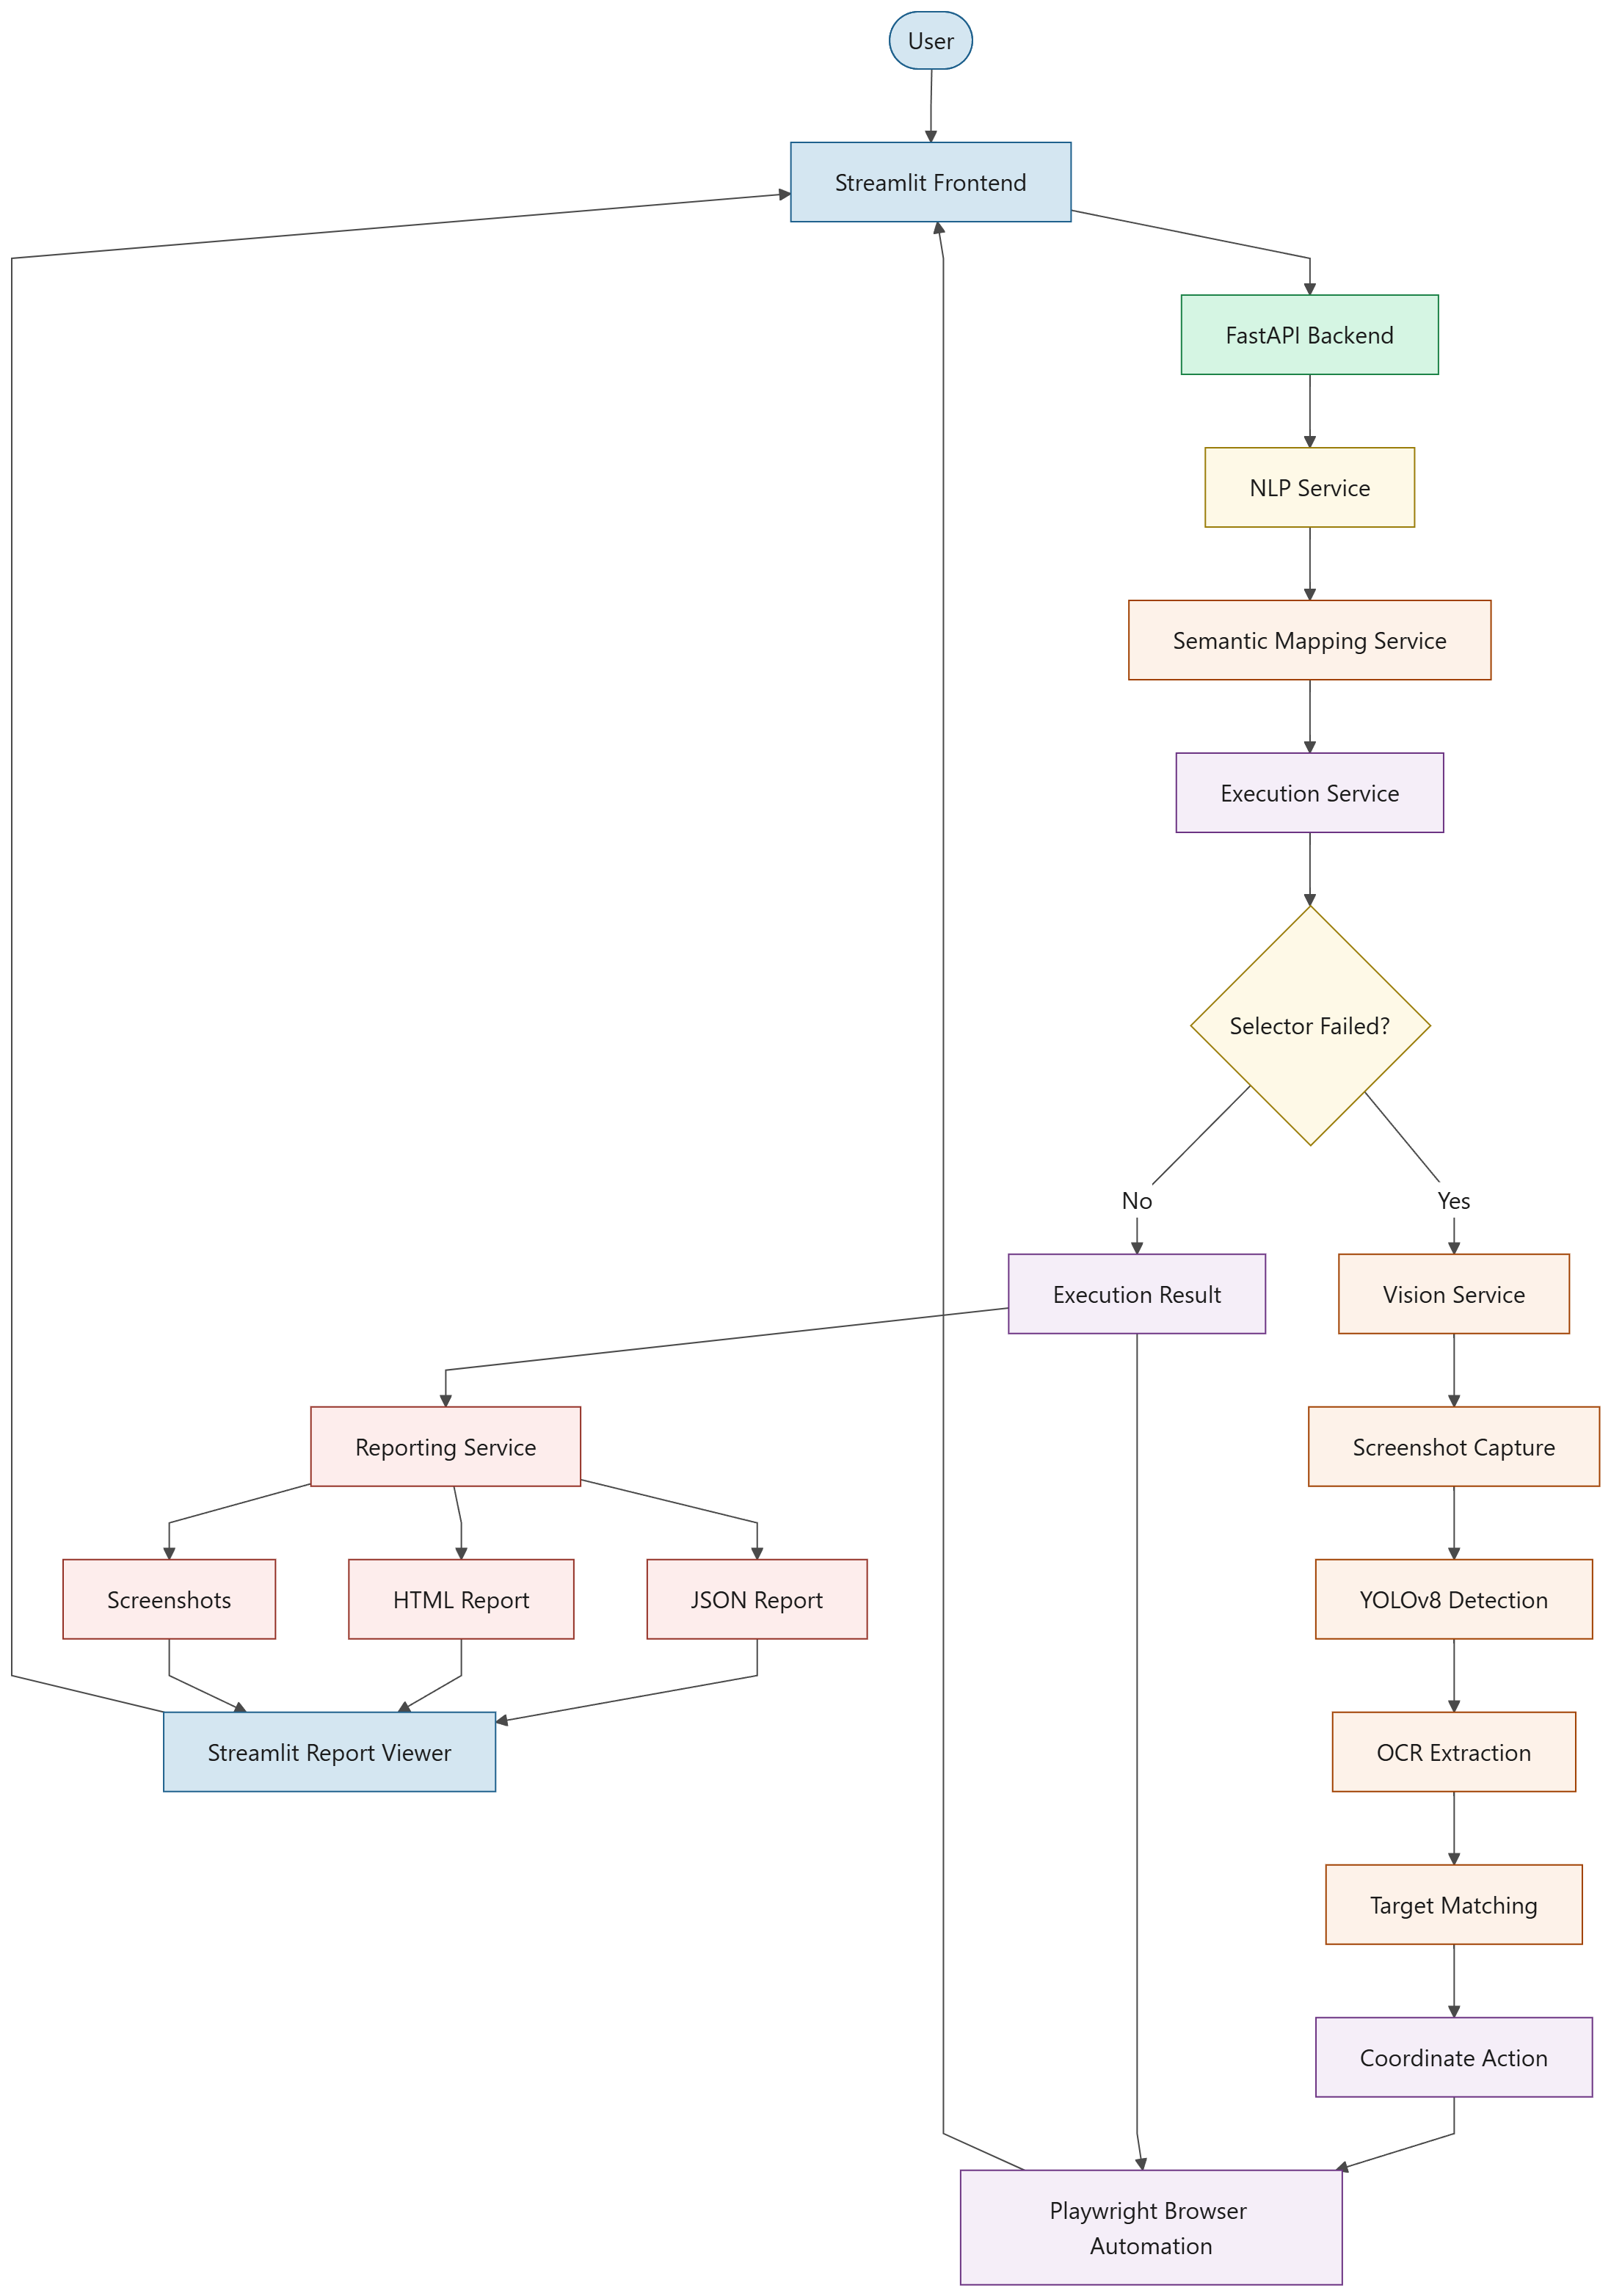
\includegraphics[width=0.9\textwidth]{global_architecture.png}
	\caption{Global architecture of VisionTest-AI}
	\label{fig:global_architecture_ch1}
\end{figure}

The solution is organized around the following modules:

\begin{itemize}
	\item \textbf{Frontend:} Streamlit interface for scenario submission, script generation, screenshot analysis, and report viewing.
	\item \textbf{Backend:} FastAPI service exposing the main API endpoints.
	\item \textbf{NLP service:} Gherkin parsing, intent classification, and entity extraction.
	\item \textbf{Semantic mapping service:} Conversion from interpreted steps to executable actions and selector candidates.
	\item \textbf{Execution service:} Playwright-based browser automation.
	\item \textbf{Vision service:} YOLOv8 and OCR-based fallback.
	\item \textbf{Reporting service:} JSON and HTML report generation.
\end{itemize}

\section{Requirements Analysis}
\label{sec:requirements_analysis_ch1}

\subsection{Functional Requirements}
\label{subsec:functional_requirements_ch1}


The functional requirements of VisionTest-AI are as follows:
\begin{itemize}
	\item[FR1:] The system shall parse Gherkin scenarios into structured steps.
	\item[FR2:] The system shall classify step intents (e.g., NAVIGATION, CLICK, INPUT, VERIFY).
	\item[FR3:] The system shall extract entities (target, value, URL) from each step.
	\item[FR4:] The system shall generate Playwright-compatible selectors and actions.
	\item[FR5:] The system shall execute browser actions via Playwright automation.
	\item[FR6:] The system shall trigger visual fallback (YOLOv8 + OCR) when selectors fail.
	\item[FR7:] The system shall capture and store screenshots during test execution.
	\item[FR8:] The system shall generate JSON and HTML execution reports for each scenario.
	\item[FR9:] The system shall provide error messages and explanations in the final report.
\end{itemize}

\subsection{Non-Functional Requirements}
\label{subsec:non_functional_requirements_ch1}


The non-functional requirements are as follows:
\begin{itemize}
	\item[NFR1:] NLP parsing response time shall be less than 5 seconds per scenario.
	\item[NFR2:] YOLOv8 inference time shall be less than 100ms per screenshot.
	\item[NFR3:] The system must be modular, maintainable, and extensible for future improvements.
	\item[NFR4:] Execution and error reports must be traceable and persistently stored.
	\item[NFR5:] The system must be usable by non-technical users (business-readable input, clear outputs).
	\item[NFR6:] The system must be robust to UI changes and provide fallback strategies.
	\item[NFR7:] The system must be open for integration with authentication, database storage, and background task queues in future versions.
\end{itemize}

\subsection{Constraints and Assumptions}
\label{subsec:constraints_assumptions_ch1}

The current version is a prototype. Its visual fallback depends on the quality of the dataset, the accuracy of YOLO detections, and the readability of OCR output. Some dynamic websites may behave differently because of popups, network speed, or anti-bot protections. The current version also does not include full PostgreSQL, Redis, authentication, or project history integration.

\section{Project Objectives}
\label{sec:project_objectives_ch1}

The functional objectives are to make Gherkin scenarios executable, reduce manual script writing, execute tests automatically, use visual fallback when needed, and generate readable execution reports. The technical objectives are to build a modular FastAPI backend~\cite{fastapi_docs}, use Pydantic schemas~\cite{pydantic_docs}, automate browsers with Playwright~\cite{playwright_docs}, integrate YOLOv8~\cite{ultralytics_yolov8_docs} and OCR, and prepare the application for future deployment improvements.

\section{Project Management Methodology}
\label{sec:methodology_ch1}

The project followed an iterative methodology inspired by Agile Scrum. This choice was suitable because the project included several uncertain components: NLP interpretation, visual detection, OCR quality, browser execution, and deployment constraints.

Figure~\ref{fig:scrum_logo} illustrates the general Scrum lifecycle used as inspiration for the project organization.

\begin{figure}[H]
	\centering
	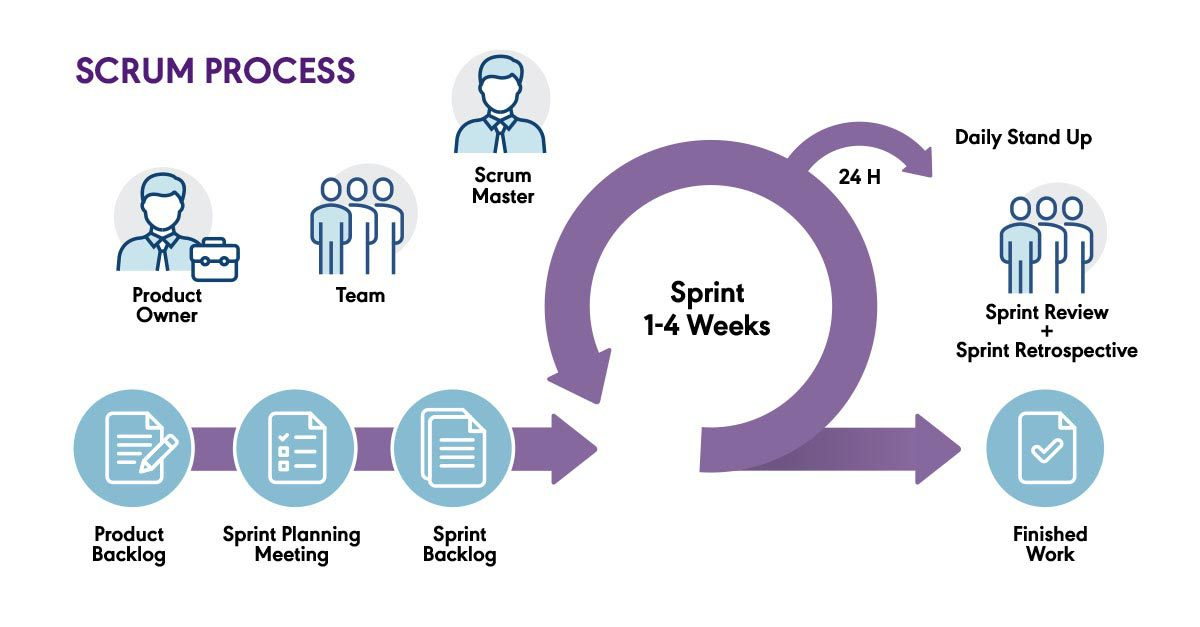
\includegraphics[width=0.55\textwidth]{Scrum_logo.jpg}
	\caption{Agile Scrum lifecycle}
	\label{fig:scrum_logo}
\end{figure}

Table~\ref{tab:sprint_planning_ch1} presents the sprint planning followed during the implementation of the prototype.

\begin{table}[H]
	\centering
	\caption{Project sprint planning}
	\label{tab:sprint_planning_ch1}
	\renewcommand{\arraystretch}{1.25}
	\small
	\begin{tabularx}{\textwidth}{|l|X|X|}
		\hline
		\rowcolor{gray!20}
		\textbf{Sprint} & \textbf{Main Objective} & \textbf{Deliverable} \\ \hline
		Sprint 1 & Problem study, requirements, and first local prototype. & Initial pipeline and backlog. \\ \hline
		Sprint 2 & NLP parsing and semantic mapping. & Structured JSON and action mapping. \\ \hline
		Sprint 3 & Dataset preparation and vision model training. & Annotated dataset and YOLO model. \\ \hline
		Sprint 4 & Execution, fallback, UI, and reporting integration. & Complete prototype. \\ \hline
	\end{tabularx}
\end{table}

Trello~\cite{trello_platform} was used for task organization, Git~\cite{git_docs} for version control, and VS Code~\cite{vscode_docs} as the main development environment.

\section{Conclusion}
\label{sec:chapter1_conclusion}

This chapter presented the general context of the project, the host organization, the testing automation problem, existing solutions, the proposed architecture, the requirements, and the project methodology. The next chapter presents the literature review needed to understand the AI and Data concepts used later in the report.

\chapter{Literature Review: Data and Artificial Intelligence Foundations}
\label{chap:literature_review}
\minitoc
\newpage

\section{Introduction}
\label{sec:ch2_intro}

Before presenting the implementation of \textbf{VisionTest-AI}, it is important to introduce the main concepts that support the project. The system combines several fields: Data Science, Machine Learning, Deep Learning, Natural Language Processing, Computer Vision, OCR, and software test automation. These fields are connected in the project because the agent must read a scenario, understand it, observe a user interface, execute actions, and produce evidence.

\subsection*{Chapter Overview}
\phantomsection
\addcontentsline{toc}{subsection}{Chapter Overview}

This chapter gives a short literature review of the AI and Data concepts used in the project. It explains the difference between Data Science, Machine Learning, Deep Learning, NLP, and Computer Vision. It also presents object detection, OCR, browser automation, and the reason why a hybrid approach is suitable for intelligent functional testing.

\section{Data Science and Artificial Intelligence}
\label{sec:data_ai_foundations}

Artificial Intelligence is a broad field that aims to build systems capable of performing tasks that usually require human intelligence. These tasks can include understanding language, recognizing objects, making decisions, or adapting to new situations. In this project, AI is used in a practical way: the system does not try to replace a QA engineer, but to assist the testing process by interpreting scenarios and detecting visual elements.

Data Science is closely related to AI because it focuses on collecting, preparing, analyzing, and using data to support decisions or build models. In \textbf{VisionTest-AI}, data appears in different forms: Gherkin text, screenshots, annotations, model outputs, logs, and generated reports. The quality of these data directly affects the reliability of the final system.

\section{Machine Learning}
\label{sec:machine_learning_review}

Machine Learning is a subfield of AI where systems learn patterns from data instead of being programmed only with fixed rules. A machine learning model receives examples during training and then uses what it learned to make predictions on new inputs.

In general, machine learning can be divided into three families:

\begin{itemize}
	\item \textbf{Supervised learning:} The model learns from labeled examples. For example, a screenshot region can be labeled as a button, input field, or link.
	\item \textbf{Unsupervised learning:} The model searches for patterns without explicit labels.
	\item \textbf{Reinforcement learning:} The model learns by interacting with an environment and receiving rewards.
\end{itemize}

This project mainly uses supervised learning in the vision part. The YOLO model is trained using annotated screenshots where UI elements are labeled with bounding boxes.

\section{Deep Learning}
\label{sec:deep_learning_review}

Deep Learning is a branch of machine learning based on neural networks with several layers. These models are effective when the input data is complex, such as text, images, audio, or video. Instead of manually defining all features, deep learning models learn useful representations from data.

Deep learning is important in this project for two reasons. First, transformer-based models such as BERT and DistilBERT are useful for language understanding~\cite{bert_paper,distilbert_paper}. Second, convolutional and detection models such as YOLO are useful for detecting visual elements in screenshots~\cite{yolo_original,ultralytics_yolov8_docs}.

\section{Natural Language Processing}
\label{sec:nlp_review}

Natural Language Processing, or NLP, is the field that studies how computers can process human language. It includes tasks such as text classification, entity extraction, question answering, translation, summarization, and semantic understanding.

In \textbf{VisionTest-AI}, NLP is used to understand Gherkin scenarios. Gherkin is readable by humans, but it must be transformed into structured actions before it can be executed by a browser. For example, the sentence:

\begin{verbatim}
	When I enter "demo@example.com" in the email field
\end{verbatim}

must be interpreted as an input action, with the value \texttt{demo@example.com}, targeting the email field.

\subsection{Rule-Based NLP}
\label{subsec:rule_based_nlp_review}

A rule-based NLP system uses predefined patterns. For example, if a sentence contains the word ``click'', the system may classify it as a click action. This approach is simple, fast, and predictable. However, it becomes limited when users write steps in different ways.

\subsection{Transformer-Based NLP}
\label{subsec:transformer_nlp_review}

Transformer models improved many NLP tasks because they can capture context in a sentence. BERT introduced a powerful language representation method based on bidirectional context~\cite{bert_paper}. DistilBERT is a lighter version designed to keep much of BERT's performance while reducing model size and inference cost~\cite{distilbert_paper}. The project uses this family of models because the system must classify user intentions from short natural language steps.

\subsection{Hybrid NLP Strategy}
\label{subsec:hybrid_nlp_review}

A fully rule-based system is too rigid, while a fully AI-based system may be difficult to control when confidence is low. For this reason, \textbf{VisionTest-AI} uses a hybrid strategy: AI helps classify intent, while deterministic rules and regular expressions are used for reliable extraction of values, URLs, and quoted text.

\section{Computer Vision}
\label{sec:computer_vision_review}

Computer Vision is the field that allows computers to analyze visual information. It includes image classification, object detection, segmentation, OCR, and visual similarity. In this project, computer vision is used to help the agent observe the user interface when selectors are not reliable.

Traditional automation tools mainly interact with the DOM. A vision-based approach adds another source of information: the screenshot. This is useful because a human tester does not need to know the DOM selector of a button; they can recognize the button visually and click it. The objective of the vision module is to bring part of this behavior into the automated system.

\section{Object Detection and YOLO}
\label{sec:yolo_review}

Object detection is a computer vision task that identifies both the class and the position of objects in an image. The output is usually a bounding box with a label and a confidence score.

YOLO, meaning ``You Only Look Once'', is a family of object detection models designed for fast detection~\cite{yolo_original}. YOLOv8, provided by Ultralytics, is widely used because it offers a practical API, efficient training, and real-time inference capabilities~\cite{ultralytics_yolov8_docs}.

In \textbf{VisionTest-AI}, YOLO is trained to detect UI elements such as:

\begin{itemize}
	\item buttons,
	\item input fields,
	\item links,
	\item dropdowns,
	\item checkboxes.
\end{itemize}

The detected bounding boxes can then be used to estimate where the agent should click or type when the selector-based approach fails.

\section{OCR and Text Extraction}
\label{sec:ocr_review}

OCR, or Optical Character Recognition, transforms text visible in an image into machine-readable text. This is important for UI testing because many elements are identified by their visible label: ``Login'', ``Submit'', ``Search'', or ``Cancel''.

Tesseract is one of the most known OCR engines~\cite{tesseract_paper,tesseract_docs}. In the project, OCR is used with screenshot regions in order to enrich visual detections. For example, YOLO may detect a button, while OCR helps determine whether this button contains the text ``Log In''.

OpenCV is also useful in the OCR pipeline because it provides image preprocessing operations such as resizing, grayscale conversion, thresholding, and cropping~\cite{opencv_library}. These operations can improve OCR readability when the image is noisy or low contrast.

\section{Behavior-Driven Development and Gherkin}
\label{sec:bdd_review}

Behavior-Driven Development, or BDD, is a development practice where expected behavior is described using examples that can be understood by both technical and non-technical stakeholders. Gherkin is commonly used in BDD because it provides a simple structure based on \texttt{Feature}, \texttt{Scenario}, \texttt{Given}, \texttt{When}, and \texttt{Then}~\cite{gherkin_reference,bdd_cucumber_book}.

This format is useful in the project because it gives the user a readable way to describe functional tests. However, Gherkin alone is not executable. The system must parse it, understand the meaning of each step, map it to an action, and execute it in the browser.

\section{Browser Automation}
\label{sec:browser_automation_review}

Browser automation frameworks allow scripts to simulate user actions. Playwright is used in the project because it supports modern browsers, automatic waiting, screenshots, and reliable end-to-end interactions~\cite{playwright_docs}. It provides the execution engine of the system.

However, Playwright still needs a way to locate elements. This is why \textbf{VisionTest-AI} generates several selector candidates and uses visual fallback when these candidates fail. The objective is not to remove Playwright, but to make its execution more adaptive.

\section{Hybrid Intelligent Testing}
\label{sec:hybrid_testing_review}

The literature and existing tools show that no single technique is sufficient alone. NLP can understand test steps but cannot click a button. Playwright can execute actions but depends on selectors. YOLO can detect UI elements but may confuse visually similar objects. OCR can read labels but may fail on small or low-contrast text.

The project therefore follows a hybrid approach:

\begin{itemize}
	\item NLP extracts the intention from the Gherkin step.
	\item Semantic mapping transforms the intention into a browser action.
	\item Playwright executes the action using selectors.
	\item YOLO and OCR provide a fallback when selectors fail.
	\item Reports store the execution evidence.
\end{itemize}

This combination is more realistic than relying on one technique. It also reflects how a human tester works: reading the scenario, understanding the expected behavior, observing the interface, performing the action, and checking the result.

\section{Conclusion}
\label{sec:ch2_conclusion}

This chapter presented the main AI and Data concepts used in \textbf{VisionTest-AI}. It introduced Data Science, Machine Learning, Deep Learning, NLP, Computer Vision, object detection, OCR, BDD, Gherkin, and browser automation. These concepts form the scientific and technical foundation of the system. The next chapter focuses on the semantic intelligence module, where Gherkin scenarios are transformed into structured actions and Playwright-compatible mappings.

\chapter{Semantic Intelligence: NLP and Mapping Module}
\label{chap:nlp_mapping}
\minitoc
\newpage

\section{Introduction}
\label{sec:ch3_intro}

After presenting the general requirements and the artificial intelligence foundations of the project, this chapter focuses on the first operational intelligence layer of \textbf{VisionTest-AI}: the NLP and semantic mapping module. Its role is to transform a functional scenario written in Gherkin into structured actions that can be executed by Playwright.

The input scenario is readable for a tester, but it is still too abstract for a browser automation engine. A sentence such as \texttt{When I click the login button} must be converted into an action type, a target, a possible selector, and optional fallback information. This chapter explains how this transformation is performed in the current prototype.

\subsection*{Chapter Overview}
\phantomsection
\addcontentsline{toc}{subsection}{Chapter Overview}

This chapter presents the NLP pipeline used in \textbf{VisionTest-AI}. It describes Gherkin parsing, intent classification, entity extraction, semantic mapping, API endpoints, generated Playwright scripts, validation examples, and the main limitations observed during testing.

\section{Objectives of the NLP Module}
\label{sec:nlp_objectives}

The NLP module was designed to solve a simple but important problem: converting business-readable test steps into automation-ready actions. In the context of the project, the module has five main objectives:

\begin{itemize}
	\item Parse Gherkin scenarios and identify features, scenarios, and steps.
	\item Detect the intent of each step, such as navigation, click, input, or verification.
	\item Extract useful entities such as target elements, values, URLs, and expected results.
	\item Convert the interpreted step into a Playwright-compatible action.
	\item Provide selector candidates that can be used first by Playwright and later by the vision fallback.
\end{itemize}

The module is therefore placed at the beginning of the complete pipeline. It receives raw text from the Streamlit interface, sends structured data to the backend services, and prepares the execution plan used by the automation layer.

Figure~\ref{fig:nlp_pipeline} represents the NLP and semantic mapping flow used in the prototype. The diagram was created by the author using Mermaid~\cite{mermaid_docs}.

\begin{figure}[H]
	\centering
	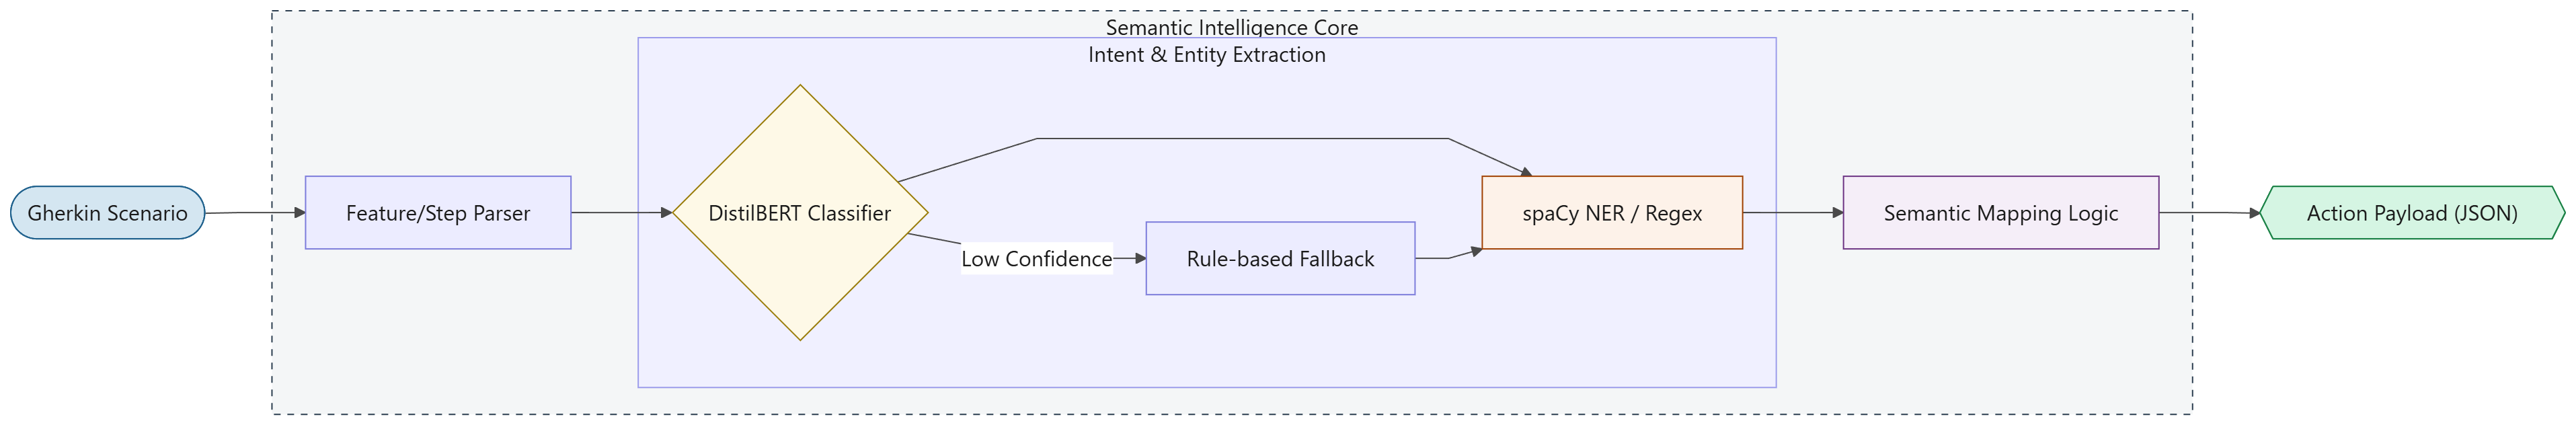
\includegraphics[width=1\textwidth]{nlp_pipeline.png}
	\caption{NLP and semantic mapping pipeline of VisionTest-AI}
	\label{fig:nlp_pipeline}
\end{figure}

\section{Gherkin Parsing}
\label{sec:gherkin_parsing}

The parser receives a raw Gherkin scenario and separates it into meaningful blocks. Gherkin was selected because it is widely used in Behavior-Driven Development and is understandable by both technical and non-technical stakeholders~\cite{gherkin_reference,bdd_cucumber_book}.

\subsection{Parsed Elements}
\label{subsec:parsed_elements}

The parser extracts three levels of information:

\begin{itemize}
	\item \textbf{Feature:} the general functionality being tested.
	\item \textbf{Scenario:} the specific test case.
	\item \textbf{Steps:} the executable instructions introduced by \texttt{Given}, \texttt{When}, \texttt{Then}, \texttt{And}, or \texttt{But}.
\end{itemize}

For example, in a login scenario, the parser identifies the authentication feature, the successful login scenario, and each step related to navigation, typing credentials, clicking a button, and checking the expected result.

Table~\ref{tab:step_extraction_example} shows how raw Gherkin lines are separated into keywords, step text, and initial interpretation.

\begin{table}[H]
	\centering
	\caption{Example of parsed Gherkin steps}
	\label{tab:step_extraction_example}
	\renewcommand{\arraystretch}{1.3}
	\small
	\begin{tabularx}{\textwidth}{|l|X|X|}
		\hline
		\rowcolor{gray!20}
		\textbf{Keyword} & \textbf{Step Text} & \textbf{Initial Interpretation} \\ \hline
		\texttt{Given} & I am on the login page & Navigation or initial context \\ \hline
		\texttt{When} & I enter admin in the username field & Input action \\ \hline
		\texttt{And} & I click the login button & Click action \\ \hline
		\texttt{Then} & I should see the dashboard & Verification action \\ \hline
	\end{tabularx}
\end{table}

\subsection{Handling \texttt{And} and \texttt{But}}
\label{subsec:and_but_steps}

The keywords \texttt{And} and \texttt{But} do not define a new action category by themselves. Their meaning depends on the previous step. For this reason, the parser keeps the original keyword for traceability, but the semantic interpretation is based on the content of the sentence. This avoids treating all \texttt{And} steps in the same way.

\section{Intent Classification}
\label{sec:intent_classification}

Intent classification identifies what the user wants to do in each step. In the current version, the system supports the most frequent actions required for functional web testing.

Table~\ref{tab:supported_intents} presents the supported intents and their corresponding automation behavior.

\begin{table}[H]
	\centering
	\caption{Supported intents in the NLP module}
	\label{tab:supported_intents}
	\renewcommand{\arraystretch}{1.3}
	\small
	\begin{tabularx}{\textwidth}{|l|l|X|}
		\hline
		\rowcolor{gray!20}
		\textbf{Intent} & \textbf{Playwright Action} & \textbf{Example Step} \\ \hline
		\texttt{NAVIGATION} & \texttt{goto} & Given I am on \texttt{https://example.com} \\ \hline
		\texttt{ACTION\_CLICK} & \texttt{click} & When I click the login button \\ \hline
		\texttt{ACTION\_TYPE} & \texttt{fill} & When I enter admin in the username field \\ \hline
		\texttt{VERIFICATION} & \texttt{expect} & Then I should see the dashboard \\ \hline
	\end{tabularx}
\end{table}

\subsection{Rule-Based First Version}
\label{subsec:rule_based_classification}

The first implementation used deterministic rules. Words such as \texttt{open}, \texttt{go to}, and \texttt{navigate} were mapped to navigation. Words such as \texttt{click}, \texttt{press}, and \texttt{select} were mapped to click actions. This approach was fast and easy to debug, but it was sensitive to wording variation.

\subsection{DistilBERT-Based Improvement}
\label{subsec:distilbert_classification}

To improve flexibility, the second version introduced a lightweight Transformer-based classifier using DistilBERT~\cite{distilbert_paper}. This model is smaller than BERT~\cite{bert_paper}, which makes it more suitable for a prototype that also includes browser automation and computer vision services.

In practice, the project uses a hybrid strategy. The model is used when the sentence is clear enough, while deterministic rules remain available as a fallback. This keeps the system understandable and avoids relying only on probabilistic output.

\subsection{Confidence Management}
\label{subsec:confidence_management}

Each interpreted step is associated with a confidence score. When the score is high, the predicted intent is accepted directly. When the score is low or when the step contains explicit patterns such as quoted values or URLs, rule-based extraction is used to protect execution reliability. This design is important because a wrong semantic decision may generate an incorrect browser action.

\section{Entity Extraction}
\label{sec:entity_extraction}

After detecting the intent, the module extracts the entities required for execution. The most important entities are the target element, the value to type, the URL, and the expected result.

Table~\ref{tab:extracted_entities} summarizes the main entities extracted from the interpreted Gherkin steps.

\begin{table}[H]
	\centering
	\caption{Main entities extracted from Gherkin steps}
	\label{tab:extracted_entities}
	\renewcommand{\arraystretch}{1.3}
	\small
	\begin{tabularx}{\textwidth}{|l|X|X|}
		\hline
		\rowcolor{gray!20}
		\textbf{Entity} & \textbf{Role} & \textbf{Example} \\ \hline
		Target & UI element to interact with. & email field, login button \\ \hline
		Value & Text to type or value to verify. & demo@example.com \\ \hline
		URL & Page to open. & https://www.facebook.com/ \\ \hline
		Element type & Expected UI component category. & input, button, link \\ \hline
	\end{tabularx}
\end{table}

\subsection{Target and Value Extraction}
\label{subsec:target_value_extraction}

The target is usually detected from expressions such as \texttt{in the email field}, \texttt{on the login button}, or \texttt{the dashboard}. The value is commonly found inside quotes or between verbs and target expressions. For example:

\begin{verbatim}
When I enter demo@example.com in the email field
\end{verbatim}

The extracted value is \texttt{demo@example.com}, and the extracted target is \texttt{email field}. The element type is inferred as \texttt{input} because the target contains the word \texttt{field}.

\subsection{Regex Fallback}
\label{subsec:regex_extraction}

Regular expressions are used for information that must be exact, especially URLs and quoted values. This fallback is intentionally simple because it protects the system from avoidable mistakes. For example, when the user writes a value between quotes, the system should not paraphrase or modify it.

\section{Semantic Mapping}
\label{sec:semantic_mapping}

Semantic mapping converts the interpreted step into a browser action. This part of the system is not only linguistic; it also prepares technical information for execution.

Table~\ref{tab:intent_action_mapping} shows how each semantic intent is translated into a Playwright-compatible method.

\begin{table}[H]
	\centering
	\caption{Mapping between semantic intents and Playwright methods}
	\label{tab:intent_action_mapping}
	\renewcommand{\arraystretch}{1.3}
	\small
	\begin{tabularx}{\textwidth}{|l|l|X|}
		\hline
		\rowcolor{gray!20}
		\textbf{Intent} & \textbf{Method} & \textbf{Generated Information} \\ \hline
		\texttt{NAVIGATION} & \texttt{goto} & URL to open \\ \hline
		\texttt{ACTION\_CLICK} & \texttt{click} & Selector candidates for a button, link, or role \\ \hline
		\texttt{ACTION\_TYPE} & \texttt{fill} & Selector candidates and input value \\ \hline
		\texttt{VERIFICATION} & \texttt{expect} & Expected text or visible element \\ \hline
	\end{tabularx}
\end{table}

\subsection{Selector Candidate Generation}
\label{subsec:selector_candidate_generation}

For each target, the mapping service generates several selector candidates. This avoids depending on one fragile selector. For an email field, candidates may include \texttt{input[name='email']}, \texttt{input\#email}, placeholders, partial name matches, partial ID matches, and label-based XPath selectors. During execution, Playwright tries the strongest selector first and can move to alternative candidates when needed.

\subsection{Preparing Vision Fallback}
\label{subsec:fallback_preparation}

The semantic output is also useful for the vision module. When a Playwright selector fails, the execution service still knows the target label and the expected element type. This information is later combined with YOLO and OCR detections to search for the element visually.

\section{API Endpoints of the NLP Module}
\label{sec:nlp_api_endpoints}

The semantic intelligence layer is exposed through FastAPI endpoints. This made it easier to test each part independently from the Streamlit interface.

\subsection{\texttt{/api/ia/parse-gherkin}}
\label{subsec:api_parse_gherkin}

This endpoint receives a raw Gherkin scenario and returns the parsed structure. It is useful for checking whether the system correctly identifies the feature, scenario, and steps before generating executable actions.

Figure~\ref{fig:parse_gherkin_request} shows an example request sent to the parsing endpoint.

\begin{figure}[H]
	\centering
	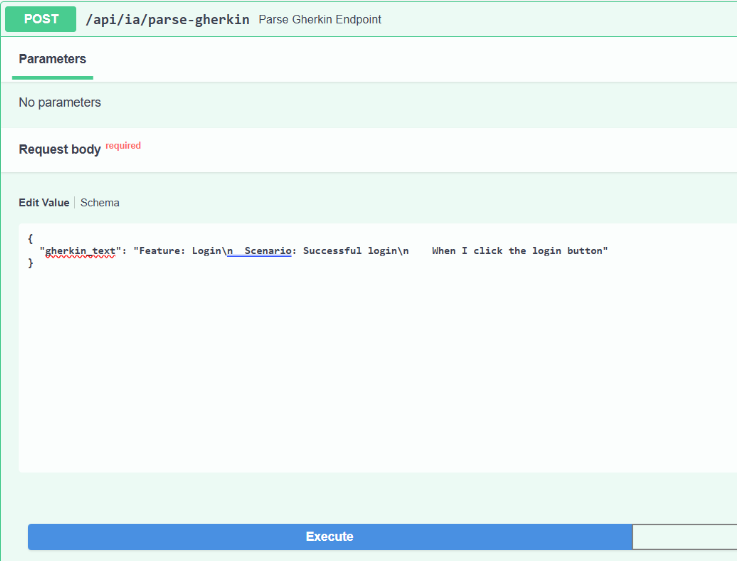
\includegraphics[width=0.87\textwidth]{parse_gherkin_request.png}
	\caption{Example request of the \texttt{/api/ia/parse-gherkin} endpoint}
	\label{fig:parse_gherkin_request}
\end{figure}

Figure~\ref{fig:parse_gherkin_response} represents the response returned by the endpoint after parsing the Gherkin scenario.

\begin{figure}[H]
	\centering
	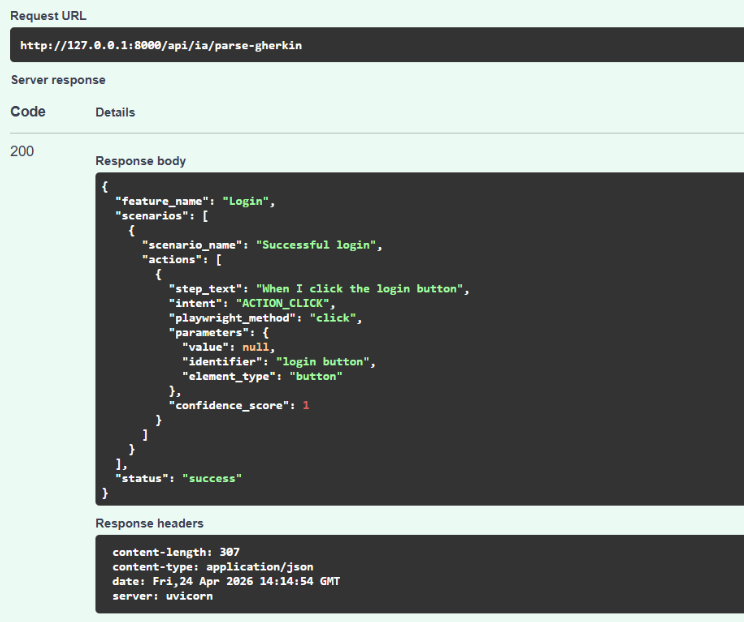
\includegraphics[width=0.87\textwidth]{parse_gherkin_response.png}
	\caption{Example response of the \texttt{/api/ia/parse-gherkin} endpoint}
	\label{fig:parse_gherkin_response}
\end{figure}

\subsection{\texttt{/api/ia/semantic-mapping}}
\label{subsec:api_semantic_mapping}

The \texttt{/api/ia/semantic-mapping} endpoint maps one raw step or one NLP payload into an actionable Playwright step. This endpoint was especially useful during debugging because it allowed each semantic decision to be tested separately.

Figure~\ref{fig:semantic_mapping_request} shows the request format used to test the semantic mapping endpoint.

\begin{figure}[H]
	\centering
	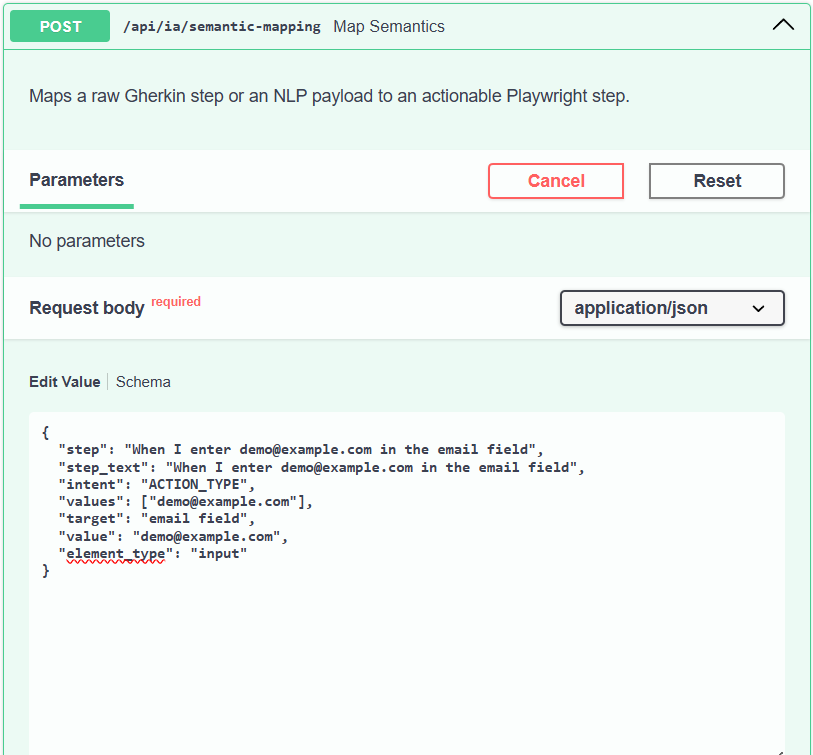
\includegraphics[width=0.87\textwidth]{semantic_mapping_request.png}
	\caption{Example request of the \texttt{/api/ia/semantic-mapping} endpoint}
	\label{fig:semantic_mapping_request}
\end{figure}

The following response shows an input step where the system extracts the typed value, detects the target as the email field, infers the element type as an input, and generates selector candidates.

\begin{lstlisting}[language=json, caption={Semantic mapping response for an input action}, label={lst:semantic_mapping_input}]
{
  "step_text": "When I enter demo@example.com in the email field",
  "intent": "ACTION_TYPE",
  "playwright_method": "input",
  "selector": "input[name='email']",
  "value": "demo@example.com",
  "element_type": "input",
  "selector_candidates": [
    "input[name='email']",
    "input#email",
    "input[placeholder*='email']",
    "input[name*='email']",
    "input[id*='email']"
  ],
  "metadata": {
    "raw_nlp": {
      "target": "email field",
      "values": ["demo@example.com"],
      "element_type": "input"
    }
  }
}
\end{lstlisting}

\subsection{\texttt{/api/ia/generate-test}}
\label{subsec:api_generate_test}

The \texttt{/api/ia/generate-test} endpoint processes a complete Gherkin scenario. Unlike the semantic mapping endpoint, which focuses on one step, this endpoint returns both a generated Playwright script and the list of interpreted actions.
\vspace{1cm}
Figure~\ref{fig:generate_test_request} shows an example request for generating a Playwright test from a complete scenario.

\begin{figure}[H]
	\centering
	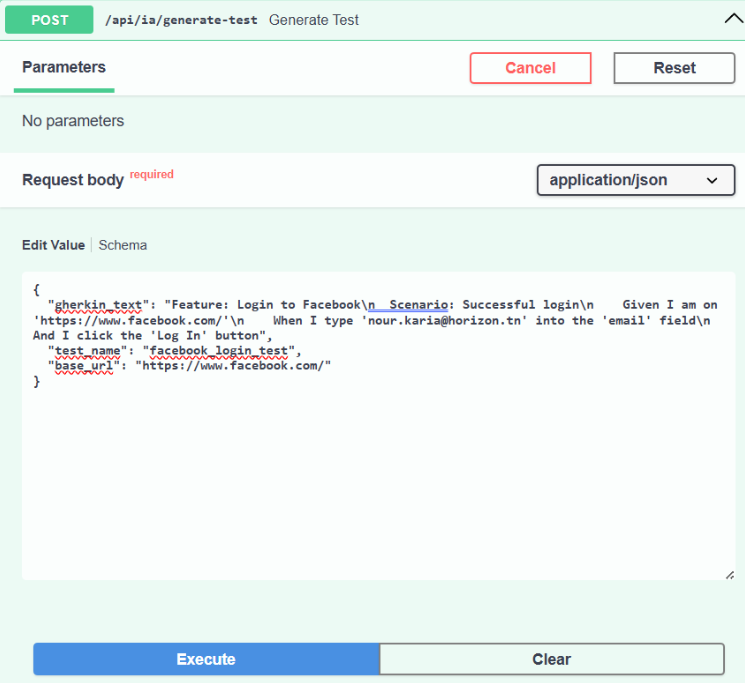
\includegraphics[width=0.85\textwidth]{generate_test_request.png}
	\caption{Example request of the \texttt{/api/ia/generate-test} endpoint}
	\label{fig:generate_test_request}
\end{figure}
\vspace{1cm}
\begin{lstlisting}[language=json, caption={Simplified response of the test generation endpoint}, label={lst:generate_test_response}]
{
  "status": "success",
  "test_name": "facebook_login_test",
  "scenarios_count": 1,
  "script": "import { test, expect } from '@playwright/test'; ...",
  "actions": [
    {
      "step_text": "Given I am on 'https://www.facebook.com/'",
      "intent": "NAVIGATION",
      "playwright_method": "navigate"
    },
    {
      "step_text": "When I type 'nour.karia@horizon.tn' into the 'email' field",
      "intent": "ACTION_TYPE",
      "playwright_method": "input"
    },
    {
      "step_text": "And I click the 'Log In' button",
      "intent": "ACTION_CLICK",
      "playwright_method": "click"
    }
  ]
}
\end{lstlisting}

\section{Generated Playwright Script}
\label{sec:generated_playwright_script}

The output of semantic mapping can be transformed into a Playwright script~\cite{playwright_docs}. This generated script gives the tester a clear view of what the system understood before execution.

\begin{lstlisting}[caption={Generated Playwright script from the Facebook login scenario}, label={lst:generated_playwright_script}]
import { test, expect } from '@playwright/test';

test("facebook_login_test", async ({ page }) => {
  await page.goto("https://www.facebook.com/");
  await page.locator("input[name='email']").first()
    .fill("nour.karia@horizon.tn");
  await page.getByRole('button', { name: "Log In",
    exact: false }).click();
});
\end{lstlisting}

\section{Validation and Results}
\label{sec:nlp_validation_results}

The validation of this module focused on realistic steps that appear frequently in functional tests: opening a page, filling a field, clicking a button, searching for a product, and checking that a message or dashboard is visible.

Table~\ref{tab:nlp_validation_examples} presents examples of correctly interpreted steps during validation.

\begin{table}[H]
	\centering
	\caption{Validation examples for the NLP and semantic mapping module}
	\label{tab:nlp_validation_examples}
	\renewcommand{\arraystretch}{1.3}
	\small
	\begin{tabularx}{\textwidth}{|X|l|X|X|}
		\hline
		\rowcolor{gray!20}
		\textbf{Input Step} & \textbf{Intent} & \textbf{Target} & \textbf{Value} \\ \hline
		Given I am on \texttt{https://example.com} & Navigation & page URL & https://example.com \\ \hline
		When I enter admin in the username field & Input & username field & admin \\ \hline
		When I click the login button & Click & login button & -- \\ \hline
		Then I should see the dashboard & Verification & dashboard & -- \\ \hline
	\end{tabularx}
\end{table}

\subsection{Observed Results}
\label{subsec:observed_results}

The tests showed that the module works well for explicit and well-structured steps. Navigation steps with URLs were extracted reliably. Input steps worked correctly when the target field and the value were both present. Click actions were also mapped correctly when the target was specific, such as \texttt{login button} or \texttt{search button}.

Table~\ref{tab:observed_mapping_results} summarizes the main mapping results observed during these tests.

\begin{table}[H]
	\centering
	\caption{Observed mapping results}
	\label{tab:observed_mapping_results}
	\renewcommand{\arraystretch}{1.3}
	\small
	\begin{tabularx}{\textwidth}{|X|X|X|}
		\hline
		\rowcolor{gray!20}
		\textbf{Case} & \textbf{Result} & \textbf{Observation} \\ \hline
		URL navigation & Successful & URLs are easy to detect with regex fallback. \\ \hline
		Input with clear field & Successful & Target and value are extracted correctly. \\ \hline
		Click with visible button name & Successful & Several selector candidates are generated. \\ \hline
		Abstract business step & Partial & The system needs more context to choose an action. \\ \hline
		Unsupported interaction & Failed & Upload, drag-and-drop, and hover are not yet mapped. \\ \hline
	\end{tabularx}
\end{table}

\subsection{Error Analysis}
\label{subsec:nlp_error_analysis}

Some errors are normal at this prototype stage. They are mainly caused by ambiguity, missing information, or unsupported actions.

Table~\ref{tab:nlp_error_analysis} presents representative NLP errors and the correction strategy considered for each case.

\begin{table}[H]
	\centering
	\caption{NLP limitations observed during validation}
	\label{tab:nlp_error_analysis}
	\renewcommand{\arraystretch}{1.3}
	\small
	\begin{tabularx}{\textwidth}{|X|X|X|}
		\hline
		\rowcolor{gray!20}
		\textbf{Input Step} & \textbf{Observed Problem} & \textbf{Correction Strategy} \\ \hline
		I authenticate with valid credentials & Too abstract for direct execution. & Ask for explicit username and password steps. \\ \hline
		I choose the first result & Depends on dynamic page state. & Add ranking logic using DOM and visual order. \\ \hline
		I upload a file & Unsupported action. & Add an upload intent and file chooser mapping. \\ \hline
		I confirm the operation & Ambiguous target. & Use popup context, OCR text, or a clearer target name. \\ \hline
	\end{tabularx}
\end{table}

\section{Limitations and Possible Improvements}
\label{sec:nlp_limitations}

The current NLP module provides a solid foundation, but it remains limited to the most common functional testing actions. Natural language can still be ambiguous, especially when the user writes business-level steps without concrete targets. The module is also mainly oriented toward English scenarios; supporting French or mixed-language scenarios would require more examples and additional extraction rules.
Future improvements include expanding the intent list, improving multilingual support, adding confidence thresholds in the interface, using previous execution reports to improve selector generation, and asking the user for confirmation when a mapping is uncertain.

\section{Conclusion}
\label{sec:ch3_conclusion}
This chapter presented the semantic intelligence layer of \textbf{VisionTest-AI}. The NLP module parses Gherkin scenarios, classifies step intents, extracts useful entities, and maps the result into Playwright-compatible actions. The validation examples show that the module works well for explicit functional steps such as navigation, input, click, and verification.

The chapter also showed why a hybrid approach is useful. Transformer-based classification improves flexibility, while deterministic fallback rules protect exact information such as URLs and typed values. The output of this module becomes the input of the execution service and prepares the target information used by the visual fallback. The next chapter presents this visual perception layer, where YOLOv8 and OCR are used to detect UI elements and support self-healing execution.

\chapter{Visual Perception and Self-Healing Execution}
\label{chap:vision_self_healing}
\minitoc
\newpage

\section{Introduction}
\label{sec:ch4_intro}

After presenting the semantic intelligence layer of \textbf{VisionTest-AI}, this chapter focuses on the visual perception layer. While the NLP module is responsible for understanding what the user wants to test, the vision module is responsible for observing the application interface and detecting the elements that can be used during execution.

Traditional web automation tools mainly interact with the Document Object Model (DOM). This approach is powerful when selectors are stable, but it becomes fragile when the interface changes, when elements are dynamically generated, or when the tested page contains components that are difficult to locate using classical selectors. For this reason, \textbf{VisionTest-AI} introduces a visual fallback mechanism based on object detection and OCR.

The objective of this chapter is to present the complete construction of the vision module. It describes the dataset preparation process, including the difficulties encountered during data collection and annotation. It then explains the training of the YOLOv8n model, the OCR pipeline, the vision API implementation, and the self-healing execution mechanism. Finally, it presents realistic observations, successful cases, failed cases, and limitations identified during testing.

\subsection*{Chapter Overview}
\phantomsection
\addcontentsline{toc}{subsection}{Chapter Overview}

This chapter follows the complete visual workflow. It starts with dataset preparation and the annotation difficulties encountered during the project. It then presents YOLOv8n training, OCR preprocessing, the vision API, the self-healing execution mechanism, and the real observations obtained during testing.

\section{Objective of the Vision Module}
\label{sec:vision_objective}

The vision module was designed to make the agent more resilient when classical selector-based automation fails. In a normal execution flow, the system first tries to interact with the page using Playwright selectors generated by the semantic mapping module. However, if these selectors fail, the system needs another way to locate the target element.

The main objective of the vision module is therefore to analyze screenshots and detect visible UI elements such as buttons, input fields, links, dropdowns, and checkboxes. Once these elements are detected, OCR is used to extract visible text and improve the matching between the semantic target and the visual elements.

The module has four main responsibilities:

\begin{itemize}
	\item Detect UI elements from screenshots using YOLOv8n.
	\item Extract visible text using OCR.
	\item Match the semantic target from the NLP module with the detected visual elements.
	\item Provide coordinates that can be used by Playwright for fallback execution.
\end{itemize}

This approach does not replace Playwright selectors. Instead, it complements them. The final execution strategy is based on two plans: Plan A uses classical selectors, while Plan B uses visual detection and coordinate-based interaction when selectors fail.

\section{Dataset Preparation: From Failed Attempts to DOM-Assisted Labeling}
\label{sec:dataset_preparation}

The preparation of the vision dataset was one of the most difficult and time-consuming parts of the project. Unlike common object detection tasks, where public datasets are often available, UI element detection requires screenshots containing realistic web components such as buttons, input fields, links, dropdowns, and checkboxes.

At the beginning of the project, the objective seemed simple: collect enough screenshots and annotate the visible interface elements. However, this phase quickly revealed several practical difficulties. Ready-made datasets were not diverse enough, manual annotation was slow, and automatic labeling tools were not immediately reliable for complex web interfaces.

For this reason, the dataset preparation evolved through several attempts before reaching the final solution based on DOM-assisted auto-labeling.

\subsection{The Challenge of Building a UI Dataset}
\label{subsec:dataset_challenge}

Building a dataset for UI element detection is different from building a dataset for natural objects. In traditional object detection, classes such as cars, persons, or animals have relatively stable visual characteristics. In web interfaces, the same class can appear in many different forms.

For example, a button can be a filled rectangle, an outlined element, a rounded component, a text-only link styled as a button, or an icon button. Similarly, input fields can have different borders, placeholders, icons, labels, and colors depending on the design system used by the website.

This visual diversity makes the dataset preparation phase critical. If the dataset is too narrow, the trained model may only recognize elements similar to those seen during training and fail on unseen websites.

\subsection{First Attempt: Searching for Ready-Made Datasets}
\label{subsec:ready_made_datasets}

The first attempt consisted of searching for existing datasets containing annotated UI elements. The goal was to save time by reusing a public dataset instead of building one from scratch.

However, this approach was not sufficient for the project. Most available datasets were either focused on mobile applications, contained synthetic interfaces, or did not include enough variation in real web layouts. Some datasets also used class names that were not aligned with the needs of \textbf{VisionTest-AI}.

The main limitation was the lack of diversity. A model trained on a limited dataset may perform well on similar screenshots, but fail when tested on websites with different themes, resolutions, layouts, or component libraries. Since the objective of the project is to support functional testing on different web applications, dataset diversity was essential.



\subsection{Second Attempt: Playwright Screenshot Generation}
\label{subsec:playwright_generation}

The second attempt was to generate screenshots using \textbf{Playwright}. This approach made it possible to open web pages automatically, capture screenshots, and create a first collection of realistic interface images.

This method was useful because it allowed the collection of screenshots from real websites and different viewport sizes. It also helped capture desktop and responsive layouts. However, screenshot generation alone did not solve the main problem: the images still needed accurate annotations.

Without reliable labels, the screenshots could not be used directly for YOLO training. This led to the next step: manual and semi-automatic annotation.



\subsection{Third Attempt: Manual Annotation with Roboflow and LabelImg}
\label{subsec:manual_annotation}

Manual annotation was tested using tools such as \textbf{Roboflow}~\cite{roboflow_docs} and \textbf{LabelImg}~\cite{labelimg_repository}. These tools allow bounding boxes to be drawn around UI elements and exported in YOLO format.

Although this approach produced accurate labels for some screenshots, it quickly became difficult to scale. Annotating each button, input field, link, and checkbox manually required a lot of time. This was especially challenging for pages containing many repeated links, menus, forms, and small clickable elements.

Another difficulty was annotation consistency. For example, deciding whether a clickable text should be labeled as a link or a button was not always obvious. Small differences in labeling rules can affect the learning process and reduce model performance.

For these reasons, manual annotation was useful for validation and correction, but it was not sufficient as the main dataset creation strategy.

Figure~\ref{fig:roboflow_manual_labeling} shows one of the manual annotation attempts performed during the dataset preparation phase.

\begin{figure}[H]
	\centering
	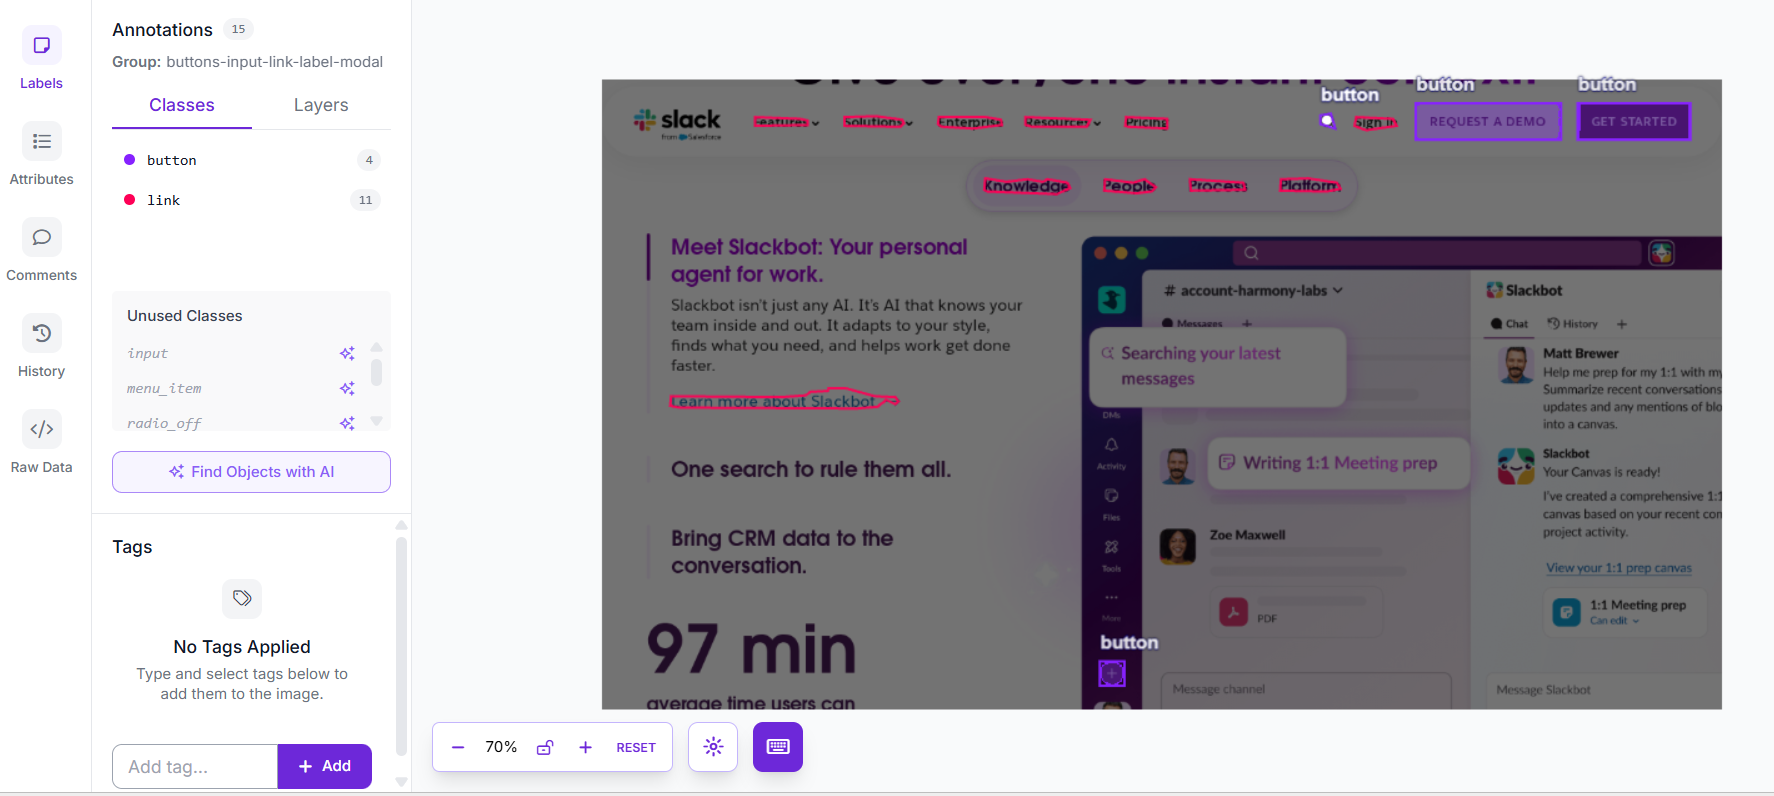
\includegraphics[width=0.95\textwidth]{roboflow_manual_labeling.png}
	\caption{Manual annotation attempt using Roboflow}
	\label{fig:roboflow_manual_labeling}
\end{figure}

\subsection{Limitations of Classic Auto-Labeling}
\label{subsec:classic_autolabeling_limits}

Auto-labeling tools were also tested to accelerate the annotation process. However, the results were not immediately reliable. In several cases, the generated boxes were inaccurate, incomplete, or assigned to the wrong class.

This problem is understandable because UI elements are visually diverse. A button may look like a simple text label, an icon, or a traditional rectangle. Input fields may appear with or without borders. Links may be mixed with paragraphs or navigation menus.

The first auto-labeling attempts therefore required significant manual correction. Instead of fully solving the problem, they showed that a more context-aware strategy was necessary.

Figure~\ref{fig:autolabeling_issue} represents an example where automatic labeling did not produce sufficiently reliable annotations.

\begin{figure}[H]
	\centering
	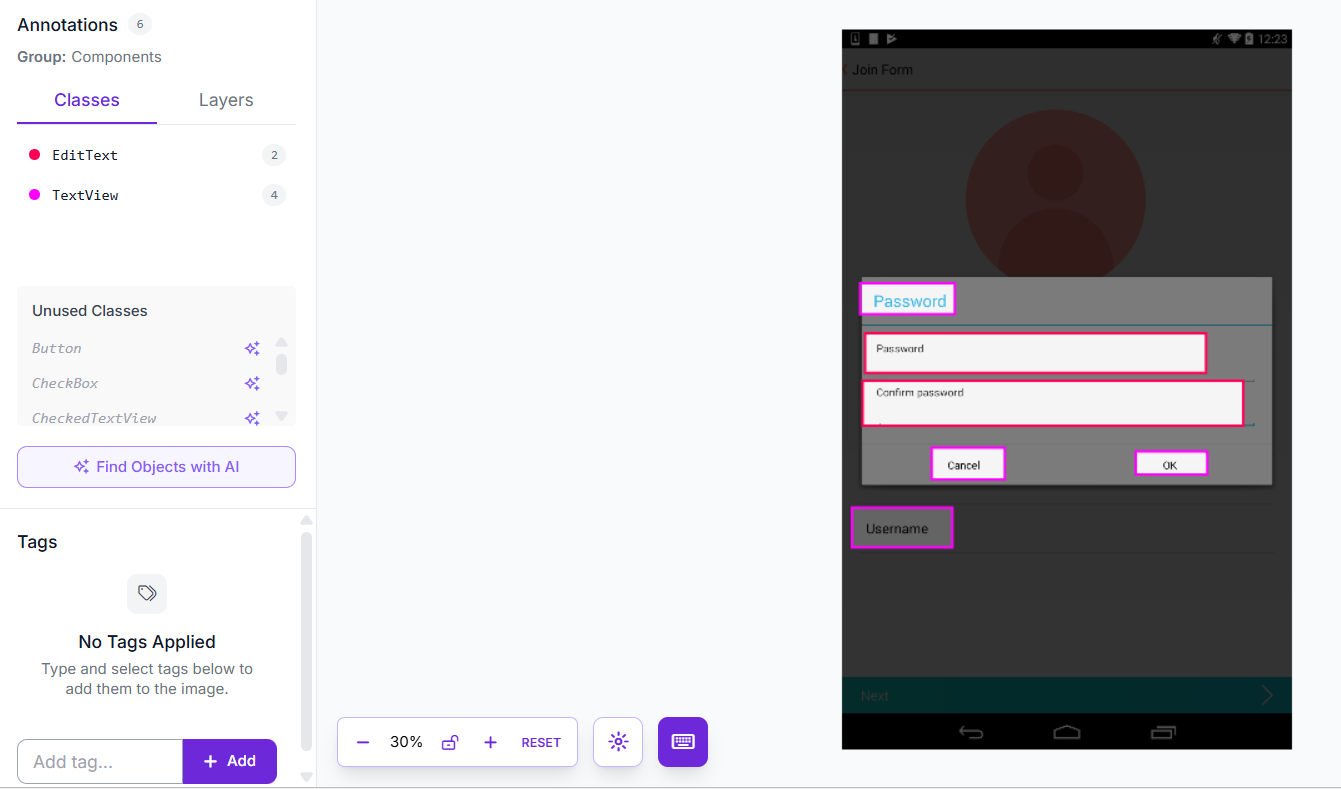
\includegraphics[width=0.95\textwidth]{autolabeling_issue.png}
	\caption{Example of incorrect or incomplete auto-labeling result}
	\label{fig:autolabeling_issue}
\end{figure}

\subsection{Final Solution: DOM-Assisted Auto-Labeling}
\label{subsec:dom_assisted_labeling}

The final solution was to use a DOM-assisted auto-labeling strategy. Instead of relying only on visual auto-labeling, the system used information extracted from the structure of the web page to generate more accurate bounding boxes.

With Playwright, it is possible to inspect DOM elements, retrieve their bounding boxes, and extract useful attributes such as tag name, role, type, placeholder, text content, and accessibility labels. This information was used to identify candidate UI elements and assign them to the appropriate classes.

For example:

\begin{itemize}
	\item \texttt{button} tags and elements with \texttt{role="button"} were labeled as buttons.
	\item \texttt{input} and \texttt{textarea} elements were labeled as input fields.
	\item \texttt{a} tags were labeled as links.
	\item \texttt{select} elements were labeled as dropdowns.
	\item \texttt{input[type="checkbox"]} elements were labeled as checkboxes.
\end{itemize}

This approach significantly improved the quality of the annotations. The labels became more consistent because they were generated from the actual structure of the page instead of being guessed only from pixels. Manual correction was still necessary in some cases, but the amount of manual work was reduced.

Figure~\ref{fig:dom_assisted_labeling} illustrates the DOM-assisted labeling strategy adopted after the first failed attempts. The diagram was created by the author using Mermaid~\cite{mermaid_docs}.

\begin{figure}[H]
	\centering
	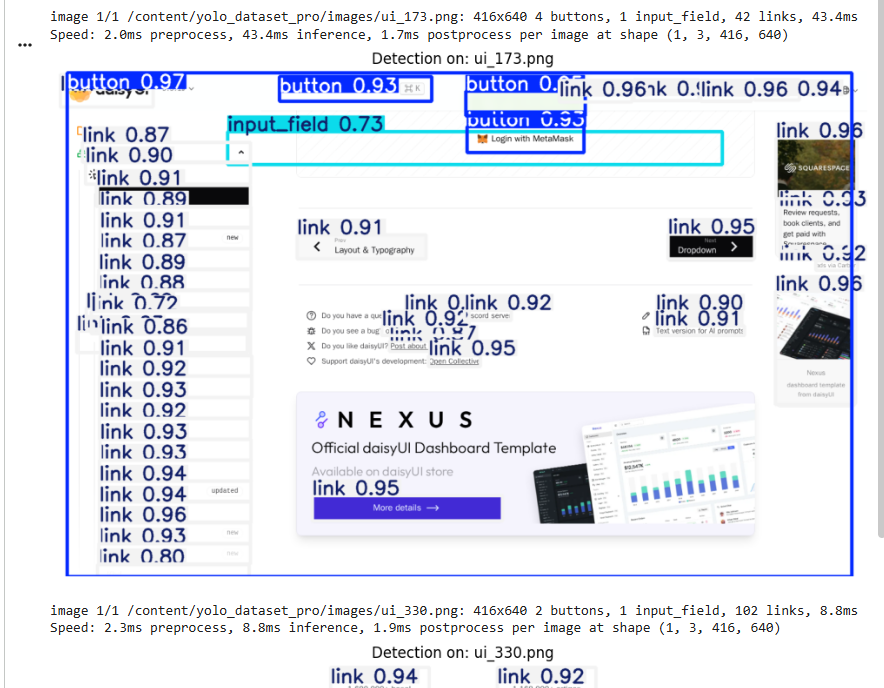
\includegraphics[width=0.95\textwidth]{dom_assisted_labeling.png}
	\caption{DOM-assisted labeling approach used to generate UI annotations}
	\label{fig:dom_assisted_labeling}
\end{figure}

\subsection{UI Element Classes}
\label{subsec:ui_element_classes}

The dataset focused on the most common interactive UI elements needed for functional testing. The selected classes were:

\begin{itemize}
	\item \textbf{Button:} Used for actions such as login, submit, search, confirm, or cancel.
	\item \textbf{Input:} Used for text fields, search bars, email fields, password fields, and text areas.
	\item \textbf{Link:} Used for navigation elements and clickable text.
	\item \textbf{Dropdown:} Used for select menus and option lists.
	\item \textbf{Checkbox:} Used for binary selections and form validation.
\end{itemize}

These classes were selected because they cover the most common user interactions in web functional testing.

Table~\ref{tab:ui_classes} describes the UI classes used to annotate the dataset.

\begin{table}[H]
	\centering
	\caption{UI classes used in the vision dataset}
	\label{tab:ui_classes}
	\renewcommand{\arraystretch}{1.35}
	\small
	\begin{tabularx}{\textwidth}{|l|X|X|}
		\hline
		\rowcolor{gray!20}
		\textbf{Class} & \textbf{Description} & \textbf{Examples} \\ \hline
		Button & Clickable component that triggers an action. & Login, Submit, Search \\ \hline
		Input & Field where the user can enter text. & Email, Password, Search field \\ \hline
		Link & Clickable text or navigation element. & Menu link, article link \\ \hline
		Dropdown & Component used to select one option from a list. & Country selector, filter menu \\ \hline
		Checkbox & Binary selection component. & Remember me, Accept terms \\ \hline
	\end{tabularx}
\end{table}

\subsection{Dataset Split and Preparation for Training}
\label{subsec:dataset_split}

After annotation, the dataset was exported in YOLO format. The images and labels were divided into training, validation, and test subsets. This split was necessary to evaluate the model on unseen data and reduce the risk of overfitting.

The training set was used to update the model weights, the validation set was used to monitor performance during training, and the test set was reserved for final evaluation.

Table~\ref{tab:dataset_split} explains the role of each dataset subset used during training and evaluation.

\begin{table}[H]
	\centering
	\caption{Dataset split used for YOLOv8n training}
	\label{tab:dataset_split}
	\renewcommand{\arraystretch}{1.35}
	\small
	\begin{tabularx}{\textwidth}{|l|X|}
		\hline
		\rowcolor{gray!20}
		\textbf{Subset} & \textbf{Role} \\ \hline
		Training set & Used to train the model and update its weights. \\ \hline
		Validation set & Used during training to monitor generalization and tune parameters. \\ \hline
		Test set & Used after training to evaluate the model on unseen examples. \\ \hline
	\end{tabularx}
\end{table}

\section{YOLOv8n Training}
\label{sec:yolov8_training}

After obtaining a more reliable annotated dataset, the next step was to train the object detection model. The objective was to detect UI elements from screenshots and return their class, confidence score, and bounding box coordinates.

\subsection{Why YOLOv8n}
\label{subsec:why_yolov8n}

The selected model was \textbf{YOLOv8n}~\cite{ultralytics_yolov8_docs,yolo_original}. This version was chosen because it offers a good compromise between speed and accuracy. Since the vision module is used during test execution, the model must be fast enough to analyze screenshots without slowing down the whole automation pipeline.

YOLOv8n is also lightweight compared to larger YOLO variants. This makes it more suitable for a prototype that may run in local environments or limited cloud environments.

Table~\ref{tab:yolo_variants} compares the YOLOv8 variants considered during model selection.

\begin{table}[H]
	\centering
	\caption{YOLOv8 variants and project positioning}
	\label{tab:yolo_variants}
	\renewcommand{\arraystretch}{1.35}
	\small
	\begin{tabularx}{\textwidth}{|l|X|X|}
		\hline
		\rowcolor{gray!20}
		\textbf{Model} & \textbf{Advantage} & \textbf{Reason for Selection} \\ \hline
		YOLOv8n & Lightweight and fast. & Selected for real-time screenshot analysis. \\ \hline
		YOLOv8s & More accurate but heavier. & Considered, but less suitable for lightweight execution. \\ \hline
		YOLOv8m/l & Higher capacity models. & Not selected due to resource constraints. \\ \hline
	\end{tabularx}
\end{table}

\subsection{Training Configuration}
\label{subsec:training_configuration}

The training configuration was selected to balance detection quality and computational cost. The model was trained using a standard image size of $640 \times 640$, which is commonly used with YOLO models and preserves enough detail for small UI elements.

Table~\ref{tab:yolo_training_config} presents the final training configuration used for YOLOv8n.

\begin{table}[H]
	\centering
	\caption{YOLOv8n training configuration}
	\label{tab:yolo_training_config}
	\renewcommand{\arraystretch}{1.35}
	\small
	\begin{tabularx}{\textwidth}{|l|l|X|}
		\hline
		\rowcolor{gray!20}
		\textbf{Parameter} & \textbf{Value} & \textbf{Justification} \\ \hline
		Model & YOLOv8n & Lightweight model suitable for real-time detection. \\ \hline
		Image size & 640 & Preserves UI details while keeping inference efficient. \\ \hline
		Epochs & 100 & Allows the model to learn UI element patterns progressively. \\ \hline
		Batch size & 16 & Balanced choice according to available memory. \\ \hline
		Task & Object detection & Required to locate UI elements with bounding boxes. \\ \hline
	\end{tabularx}
\end{table}

\subsection{Loss Function Analysis}
\label{subsec:loss_analysis}

During training, several losses were monitored:

\begin{itemize}
	\item \textbf{Box loss:} Measures the quality of bounding box localization.
	\item \textbf{Class loss:} Measures the quality of class prediction.
	\item \textbf{DFL loss:} Helps refine bounding box boundaries.
\end{itemize}

For this project, box localization is particularly important. If a button is detected but the bounding box is inaccurate, the fallback coordinate click may be placed outside the real element. This would reduce the reliability of the self-healing mechanism.

\subsection{Training Metrics}
\label{subsec:training_metrics}

After training, the model performance was analyzed using the metrics generated by YOLOv8. These metrics include training losses, validation losses, precision, recall, and mean Average Precision.

Figure~\ref{fig:training_results} represents the training metrics obtained after the YOLOv8n training process.

\begin{figure}[H]
	\centering
	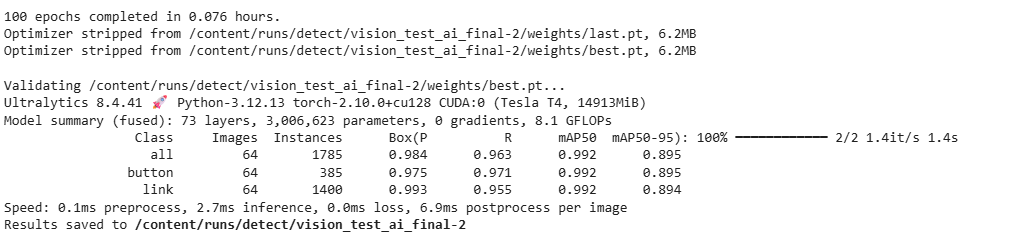
\includegraphics[width=1.0\textwidth]{results.png}
	\caption{YOLOv8n training metrics: loss curves, precision, recall, and mAP evolution}
	\label{fig:training_results}
\end{figure}

The curves provide insight into the behavior of the model during training. A decreasing loss indicates that the model is learning useful visual patterns, while stable validation metrics suggest that the model is not only memorizing the training examples.

\subsection{Model Evaluation}
\label{subsec:model_evaluation}

The evaluation focused on whether the model could correctly detect the most important UI components for functional testing. Buttons and input fields were especially important because they are directly used during click and input actions.

The results showed that the model was able to detect several common components correctly. However, some classes remained more difficult, especially when they appeared in small sizes, low contrast, or visually similar styles.

Figure~\ref{fig:confusion_matrix} shows the confusion matrix used to analyze the model behavior across UI classes.

\begin{figure}[H]
	\centering
	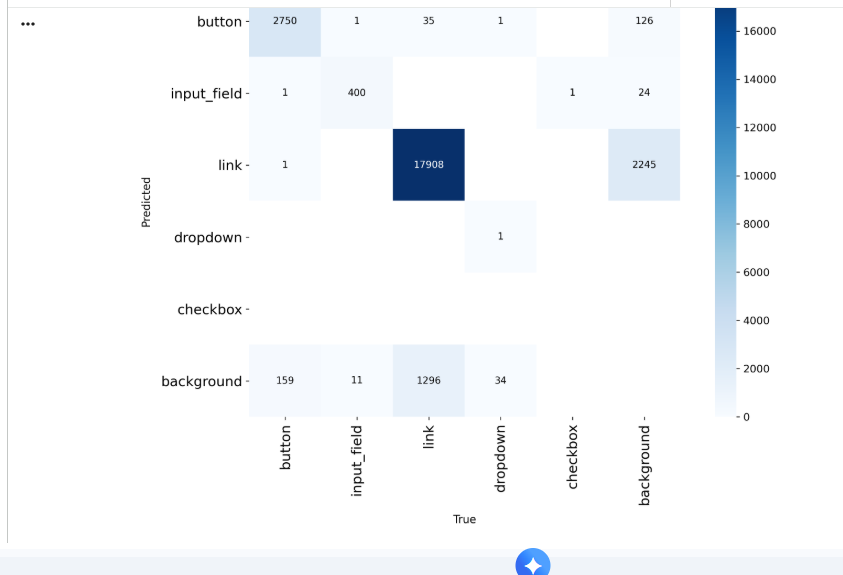
\includegraphics[width=0.85\textwidth]{confusion_matrix.png}
	\caption{Confusion matrix of the trained YOLOv8n model}
	\label{fig:confusion_matrix}
\end{figure}

\section{OCR Pipeline}
\label{sec:ocr_pipeline}

Object detection alone is not enough for self-healing execution. YOLO can detect that an element is a button or an input field, but it does not always know which button is the correct one. For example, a page can contain several buttons such as \textit{Login}, \textit{Cancel}, \textit{Search}, and \textit{Submit}.

For this reason, OCR was integrated into the vision pipeline. OCR helps extract visible text from the screenshot and associate it with detected elements.

\subsection{Role of OCR in the Vision Module}
\label{subsec:ocr_role}

The role of OCR is to enrich visual detections with textual information. When the NLP module asks for the \texttt{login button}, the vision module can use OCR to find detected buttons whose visible text is close to \texttt{login}.

This improves the matching process between the semantic target and the visual candidates.

\subsection{OpenCV Preprocessing}
\label{subsec:opencv_preprocessing}

Before applying OCR, screenshots can be preprocessed using \textbf{OpenCV}~\cite{opencv_library}. Preprocessing improves the readability of text and may include grayscale conversion, thresholding, noise reduction, or cropping detected regions.

The objective is not to modify the interface, but to make the text easier for OCR to read.

\subsection{Tesseract OCR}
\label{subsec:tesseract_ocr}

\textbf{Tesseract OCR}~\cite{tesseract_paper,tesseract_docs} was used to extract text from screenshots and detected regions. The extracted text is then cleaned and normalized before being compared with the target extracted from the Gherkin step.

OCR is especially useful for buttons, links, and labels. However, it can be less reliable when the text is small, blurred, partially hidden, or rendered with low contrast.

\subsection{Text Cleaning and Matching}
\label{subsec:text_cleaning_matching}

After OCR extraction, the text is cleaned by removing unnecessary spaces, normalizing case, and filtering irrelevant characters. The cleaned text is then compared with the semantic target using simple matching techniques.

For example, if the target is \texttt{login button}, the matching process prioritizes detections containing the text \texttt{login}. This helps the vision module choose the most relevant element among several candidates.

\section{Vision API Implementation}
\label{sec:vision_api}

The vision module is exposed through API endpoints that allow screenshots to be analyzed and detections to be returned in JSON format.

\subsection{\texttt{/api/ia/analyze-screenshot}}
\label{subsec:api_analyze_screenshot}

The \texttt{/api/ia/analyze-screenshot} endpoint receives a screenshot and applies the vision pipeline. It returns detected UI elements, bounding boxes, confidence scores, and OCR information when available.

This endpoint is useful for testing the vision module independently from the full execution pipeline.

Figure~\ref{fig:analyze_screenshot_request} shows an example request sent to the screenshot analysis endpoint.

\begin{figure}[H]
	\centering
	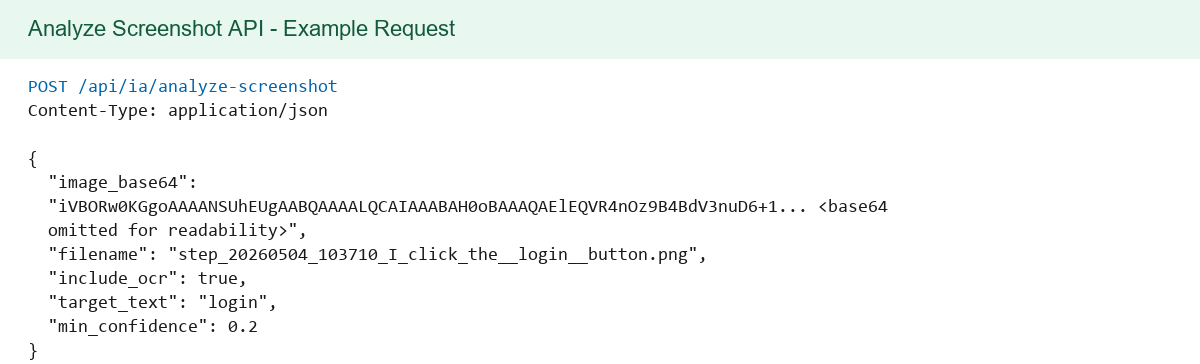
\includegraphics[width=0.95\textwidth]{analyze_screenshot_request.png}
	\caption{Example request of the \texttt{/api/ia/analyze-screenshot} endpoint}
	\label{fig:analyze_screenshot_request}
\end{figure}

\subsection{Screenshot Input}
\label{subsec:screenshot_input}

The screenshot can come from different sources. It can be uploaded by the user, captured during execution, or generated by Playwright when a selector fails.

In the self-healing process, screenshots are usually captured automatically by the execution service at the moment of failure.

\subsection{Bounding Box Detection}
\label{subsec:bounding_box_detection}

After receiving the screenshot, the YOLOv8n model detects UI elements and returns bounding boxes. Each bounding box contains the position and size of the detected element.

A typical detection includes:

\begin{itemize}
	\item Class name.
	\item Confidence score.
	\item Bounding box coordinates.
	\item Optional OCR text.
\end{itemize}

\begin{lstlisting}[caption={Simplified vision detection response}, label={lst:vision_detection_response}]
	{
		"status": "success",
		"detections": [
		{
			"class_name": "button",
			"confidence": 0.86,
			"bbox": [420, 310, 520, 350],
			"text": "Log In"
		},
		{
			"class_name": "input",
			"confidence": 0.91,
			"bbox": [250, 180, 540, 220],
			"text": "Email"
		}
		]
	}
\end{lstlisting}

\subsection{OCR Enrichment}
\label{subsec:ocr_enrichment}

After detecting bounding boxes, OCR is applied to selected regions in order to extract visible text. This allows the system to associate semantic labels with visual elements.

For example, a detected button with OCR text \texttt{Log In} becomes a stronger candidate when the target is \texttt{login button}.

\subsection{Returned JSON Structure}
\label{subsec:vision_json_structure}

The returned JSON structure is designed to be consumed by the execution service. It provides enough information to select a candidate and perform a coordinate-based action if needed.

The center of the bounding box can be used as the click coordinate:

\[
x_{center} = \frac{x_{min} + x_{max}}{2}
\]

\[
y_{center} = \frac{y_{min} + y_{max}}{2}
\]

This coordinate is then passed to Playwright for fallback execution.

\section{Self-Healing Execution}
\label{sec:self_healing_execution}

The self-healing mechanism is one of the most important parts of \textbf{VisionTest-AI}. Its purpose is to continue execution when the primary selector-based strategy fails.

\subsection{Plan A: Playwright Selector Execution}
\label{subsec:plan_a}

Plan A is the default execution strategy. The system uses selector candidates generated by the semantic mapping module and tries to execute the action with Playwright.

For example, for the step:

\begin{verbatim}
	When I click the login button
\end{verbatim}

the system may try selectors such as:

\begin{itemize}
	\item \texttt{button[name='login']}
	\item \texttt{button[type='submit']}
	\item \texttt{[role='button']:has-text('Log in')}
	\item \texttt{text='login'}
\end{itemize}

If one selector succeeds, the step is considered passed.

\subsection{Plan B: YOLO + OCR + Coordinate-Based Action}
\label{subsec:plan_b}

If Plan A fails, the system activates Plan B. In this case, the execution service captures a screenshot of the current page and sends it to the vision module.

The vision module detects UI elements, extracts OCR text, ranks candidates, and returns the most relevant element. The execution service then uses the center of the selected bounding box to perform a coordinate-based action.

This process allows the system to recover from selector failures in some cases.

Figure~\ref{fig:fallback_example} represents a screenshot captured during a fallback execution, when selector-based execution was not sufficient.

\begin{figure}[H]
	\centering
	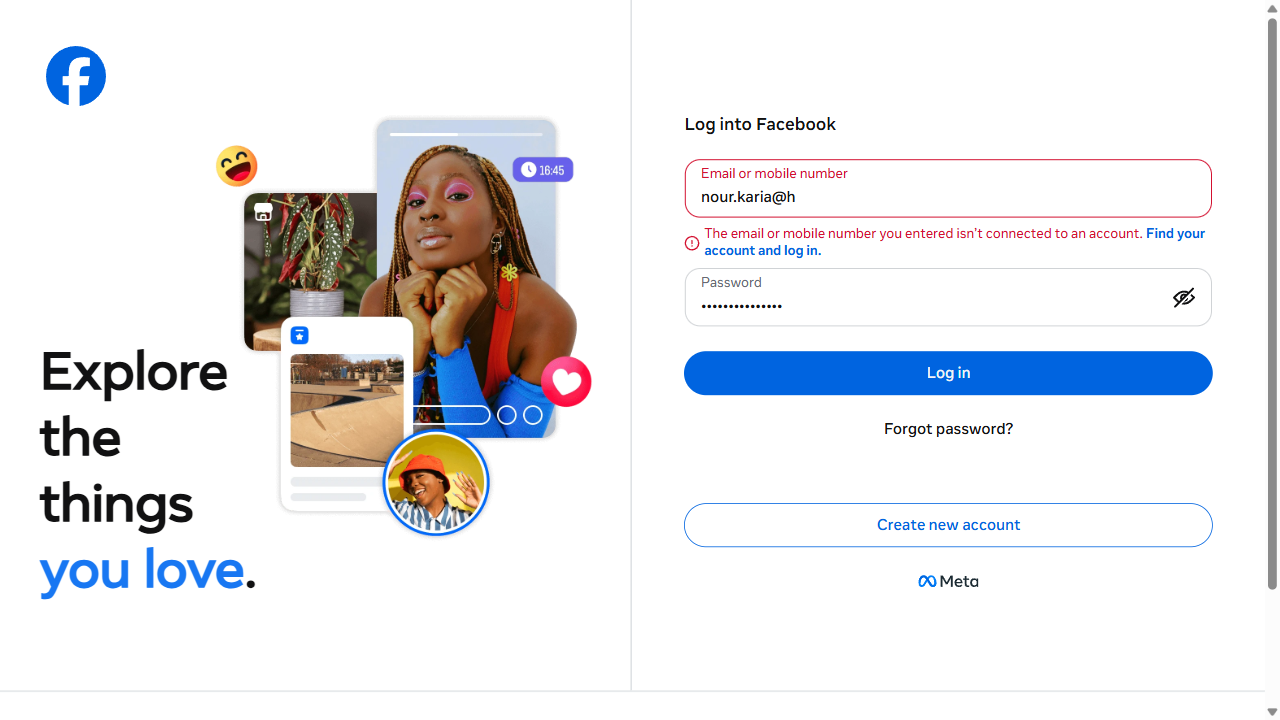
\includegraphics[width=0.95\textwidth]{fallback_example.png}
	\caption{Screenshot captured during a fallback execution}
	\label{fig:fallback_example}
\end{figure}

\subsection{Retry Mechanism}
\label{subsec:retry_mechanism}

Web interfaces are often dynamic. Elements may appear after a delay, popups may block interactions, and content may load asynchronously. For this reason, the execution service includes a retry mechanism.

If an action fails, the system can wait briefly, capture a new screenshot, and try again. This improves robustness in pages where the state changes after loading.

\subsection{Popup and Dialog Handling}
\label{subsec:popup_handling}

During testing, popups and dialogs were frequently encountered, especially cookie consent dialogs or login overlays. These elements can block the target UI element and cause execution failure.

To handle this, the system attempts to detect common popup buttons such as \texttt{Accept}, \texttt{Allow}, \texttt{Close}, or \texttt{OK}. When such elements are detected, the system can interact with them before continuing the original test.

\section{Results and Observations}
\label{sec:vision_results_observations}

The vision module was evaluated through both isolated screenshot analysis and full execution scenarios. The objective was not to claim perfect detection, but to verify whether the module could support the self-healing mechanism in realistic cases.

\subsection{Successful Detection Cases}
\label{subsec:successful_detection_cases}

The model produced good results on common UI elements such as buttons and input fields. Detection was especially reliable when the elements had clear borders, sufficient contrast, and standard layouts.

Figure~\ref{fig:vision_detection_result} shows an example of a successful visual detection result.

\begin{figure}[H]
	\centering
	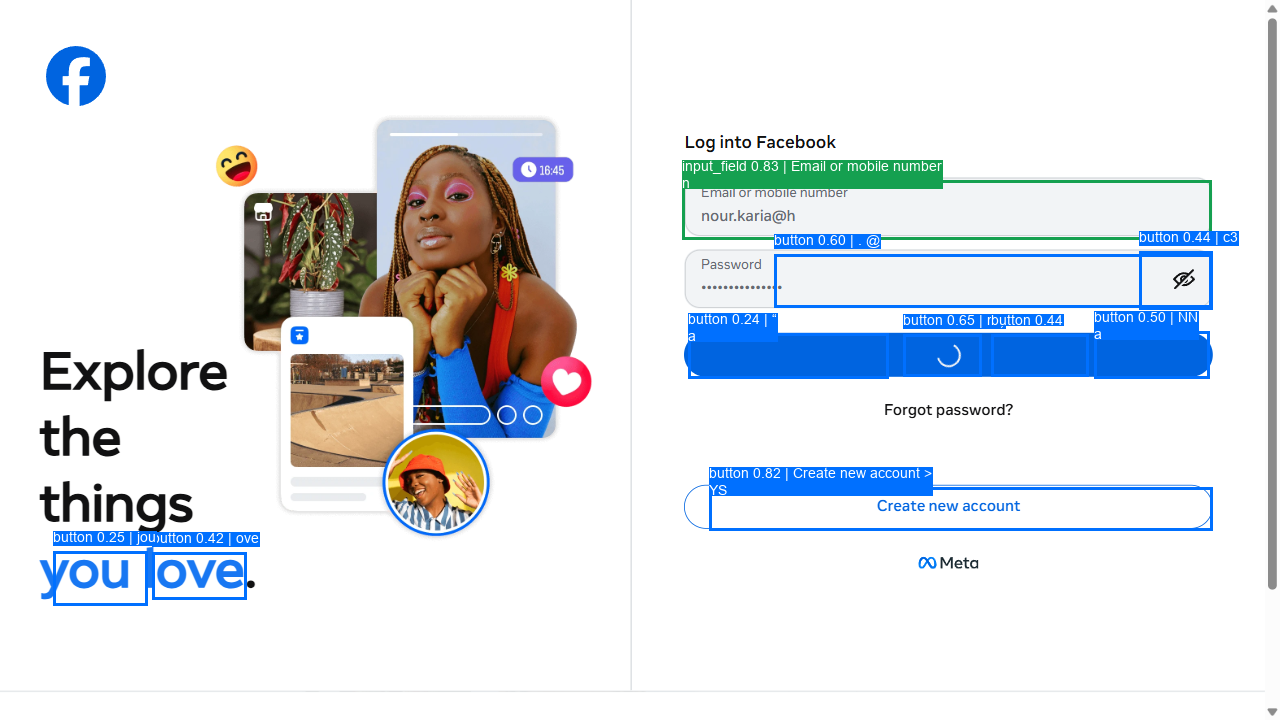
\includegraphics[width=0.95\textwidth]{vision_detection_result.png}
	\caption{Example of successful UI element detection}
	\label{fig:vision_detection_result}
\end{figure}

\subsection{Successful Self-Healing Cases}
\label{subsec:successful_self_healing_cases}

The self-healing mechanism was useful when generated selectors failed but the target element was still visible on the screen. In these cases, the system used screenshot analysis and coordinate-based execution to continue the test.

For example, if the selector for a login button failed because the HTML attributes changed, the vision module could still detect the visible button and provide its coordinates.

Table~\ref{tab:self_healing_success} summarizes examples where the visual fallback helped continue execution after a selector failure.

\begin{table}[H]
	\centering
	\caption{Examples of successful self-healing situations}
	\label{tab:self_healing_success}
	\renewcommand{\arraystretch}{1.35}
	\small
	\begin{tabularx}{\textwidth}{|X|X|X|}
		\hline
		\rowcolor{gray!20}
		\textbf{Situation} & \textbf{Plan A Result} & \textbf{Plan B Result} \\ \hline
		Login button selector not found & Failed selector lookup & Button detected visually and clicked by coordinates \\ \hline
		Search input selector changed & Fill action failed & Input field detected and filled using fallback strategy \\ \hline
		Cookie popup blocked page & Main action blocked & Popup button detected and handled before retry \\ \hline
	\end{tabularx}
\end{table}

\subsection{Failed Cases}
\label{subsec:failed_cases}

Some failures were still observed. The most common causes were OCR errors, low contrast, overlapping elements, and ambiguous targets.

For example, if several buttons had similar text or no visible text, the system could choose the wrong candidate. Similarly, if OCR failed to read the label of a small button, the ranking process became less reliable.

Table~\ref{tab:vision_failed_cases} presents the main failed cases observed during the validation of the vision module.

\begin{table}[H]
	\centering
	\caption{Observed failed cases in the vision module}
	\label{tab:vision_failed_cases}
	\renewcommand{\arraystretch}{1.35}
	\small
	\begin{tabularx}{\textwidth}{|X|X|X|}
		\hline
		\rowcolor{gray!20}
		\textbf{Failure Case} & \textbf{Cause} & \textbf{Possible Improvement} \\ \hline
		Small icon button not detected & Element too small or visually similar to background & Add more icon examples and increase dataset diversity \\ \hline
		Wrong button selected & Several candidates had similar visual/textual features & Improve ranking with DOM context and OCR confidence \\ \hline
		Text not extracted correctly & OCR failed due to low contrast or small font & Improve preprocessing and OCR configuration \\ \hline
		Dropdown not detected reliably & Limited number of dropdown examples in dataset & Add more annotated dropdown samples \\ \hline
	\end{tabularx}
\end{table}

\subsection{Error Analysis}
\label{subsec:vision_error_analysis}

The error analysis shows that the vision module is useful as a fallback mechanism, but it should not be considered a complete replacement for selector-based automation. Playwright selectors remain more precise when the DOM is accessible and stable. The vision module becomes valuable when selectors fail or when the visual state of the page provides stronger information than the HTML structure.

The main improvement needed is dataset diversity. More examples of different UI styles, themes, screen sizes, and component libraries would improve the model's ability to generalize.

\section{Conclusion}
\label{sec:ch4_conclusion}

This chapter presented the visual perception and self-healing execution layer of \textbf{VisionTest-AI}. It first described the dataset preparation process, which evolved from searching for ready-made datasets and manual annotation attempts to a more reliable DOM-assisted auto-labeling approach.

The chapter then presented the YOLOv8n training phase, including the choice of model, training configuration, loss analysis, and evaluation metrics. OCR was also integrated to enrich visual detections with text information and improve target matching.

Finally, the chapter explained the self-healing execution mechanism based on Plan A and Plan B. Plan A relies on Playwright selectors, while Plan B uses YOLO, OCR, and coordinate-based actions when selectors fail.

The results showed that the vision module can improve robustness in some realistic situations, especially when the target element remains visible but selector-based execution fails. However, the module still has limitations related to dataset diversity, OCR reliability, and ambiguous visual targets. The next chapter will focus on the complete system integration, reporting, deployment attempts, and final results of the project.

\chapter{Integration, Reporting, Deployment and Final Results}
\label{chap:integration_results}
\minitoc
\newpage

\section{Introduction}
\label{sec:ch5_intro}

After presenting the semantic intelligence module and the visual perception layer, this chapter focuses on the complete integration of \textbf{VisionTest-AI}. The objective is to show how the different modules work together to form a functional testing pipeline, from the submission of a Gherkin scenario to the generation of execution reports.

This chapter presents the full system workflow, the backend implementation, the reporting system, the user interface, deployment attempts, testing strategy, and final results. It also discusses the limitations observed during the project and the possible improvements for future versions.

Unlike the previous chapters, which focused on specific modules, this chapter provides a global view of the final prototype. It shows how NLP parsing, semantic mapping, Playwright execution, vision fallback, and report generation are connected inside the same system.

\subsection*{Chapter Overview}
\phantomsection
\addcontentsline{toc}{subsection}{Chapter Overview}

This chapter presents the final prototype from an engineering point of view. It describes the complete pipeline, backend routers and services, reporting system, Streamlit interface, deployment attempts, validation strategy, actual results, limitations, and perspectives.

\section{Complete Pipeline Integration}
\label{sec:complete_pipeline}

The complete pipeline of \textbf{VisionTest-AI} starts with a Gherkin scenario written by the user and ends with structured execution reports. The system was designed as a modular pipeline where each component has a specific responsibility.

\subsection{User Submits a Gherkin Scenario}
\label{subsec:user_submits_gherkin}

The first step begins when the user submits a Gherkin scenario through the interface. The scenario describes the functional behavior to test using readable steps such as \texttt{Given}, \texttt{When}, and \texttt{Then}.

An example scenario is:

\begin{verbatim}
	Feature: Facebook login
	
	Scenario: Invalid login attempt
	Given I am on 'https://www.facebook.com/'
	When I type 'nour.karia@horizon.tn' into the 'email' field
	And I type 'facebook1234' into the 'password' field
	And I click the 'Log In' button
	Then I should see the error message
\end{verbatim}

This scenario is understandable by a human tester, but it must be transformed into structured actions before execution.

\subsection{NLP Parsing and Semantic Mapping}
\label{subsec:nlp_mapping_integration}

After receiving the scenario, the backend sends it to the NLP module. This module extracts the feature name, scenario name, and steps. Each step is then analyzed to identify the intent, target, value, and element type.

The semantic mapping module converts these interpreted steps into executable actions. For example, an input step is mapped to a Playwright \texttt{fill} action, while a click step is mapped to a Playwright \texttt{click} action.

\subsection{Playwright Execution}
\label{subsec:playwright_execution_integration}

The execution service uses Playwright to interact with the browser. It opens the target page, executes each action, captures screenshots, and records the status of every step.

The primary execution strategy is selector-based. This means that the system first tries to interact with elements using generated selector candidates such as role selectors, text selectors, CSS selectors, or XPath expressions.

\subsection{Vision Fallback When Selectors Fail}
\label{subsec:vision_fallback_integration}

If all selector candidates fail, the system activates the visual fallback strategy. In this case, the execution service captures a screenshot of the current page and sends it to the vision module.

The vision module analyzes the screenshot using YOLOv8n and OCR. It detects UI elements, extracts visible text, ranks possible candidates, and returns coordinates that can be used for a fallback action.

This mechanism is called self-healing execution because it allows the system to recover from some selector failures.

\subsection{Report Generation}
\label{subsec:report_generation_pipeline}

At the end of execution, the reporting service generates structured reports. These reports contain the execution status, the list of executed steps, screenshots, errors, execution duration, and the strategy used for each step.

Two report formats are generated:

\begin{itemize}
	\item \textbf{JSON report:} Used for structured storage and future processing.
	\item \textbf{HTML report:} Used for human-readable visualization.
\end{itemize}

Figure~\ref{fig:complete_pipeline} represents the complete execution pipeline of \textbf{VisionTest-AI}, from scenario submission to report generation. The diagram was created by the author using Mermaid~\cite{mermaid_docs}.

\begin{figure}[H]
	\centering
	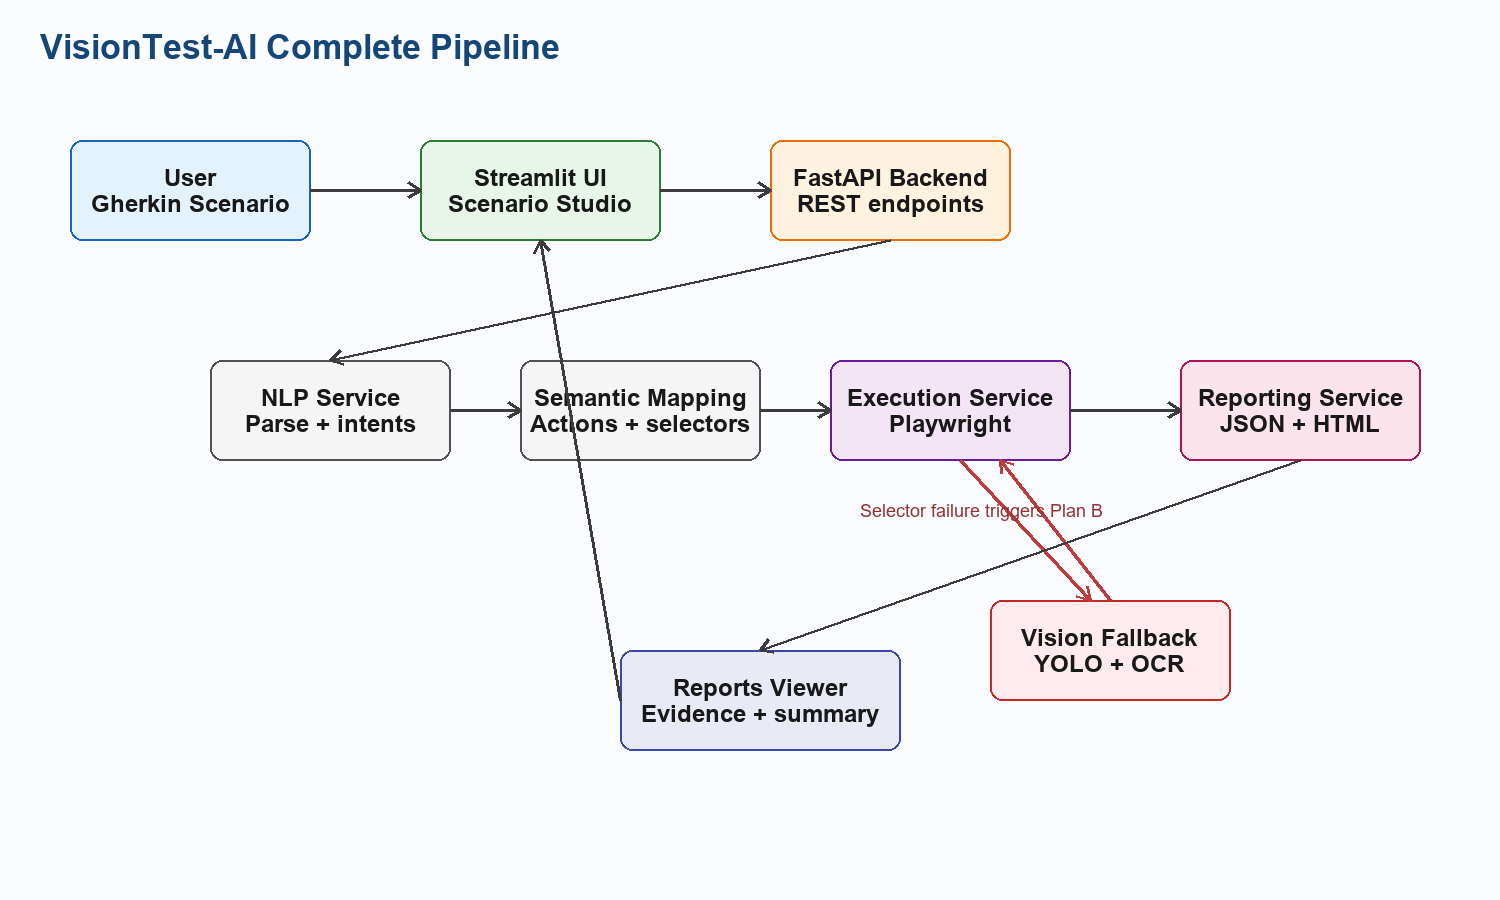
\includegraphics[width=0.95\textwidth]{complete_pipeline.png}
	\caption{Complete execution pipeline of VisionTest-AI}
	\label{fig:complete_pipeline}
\end{figure}

\section{Backend Implementation}
\label{sec:backend_implementation}

The backend was implemented using \textbf{FastAPI}~\cite{fastapi_docs}. It exposes the different services of the system through REST API endpoints and coordinates the communication between the NLP, mapping, execution, vision, and reporting modules.

\subsection{FastAPI Routers}
\label{subsec:fastapi_routers}

The backend is organized using routers. Each router is responsible for a specific part of the system.

Table~\ref{tab:fastapi_routers} summarizes the main FastAPI routers implemented in the backend.

\begin{table}[H]
	\centering
	\caption{Main FastAPI routers of VisionTest-AI}
	\label{tab:fastapi_routers}
	\renewcommand{\arraystretch}{1.35}
	\small
	\begin{tabularx}{\textwidth}{|l|X|}
		\hline
		\rowcolor{gray!20}
		\textbf{Router} & \textbf{Responsibility} \\ \hline
		\texttt{nlp\_parsing.py} & Parses Gherkin scenarios and returns structured actions. \\ \hline
		\texttt{semantic\_mapping.py} & Maps interpreted steps to executable Playwright actions. \\ \hline
		\texttt{test\_generation.py} & Generates Playwright scripts from Gherkin scenarios. \\ \hline
		\texttt{test\_execution.py} & Executes test scenarios using Playwright. \\ \hline
		\texttt{ql\_detection.py} & Analyzes screenshots and detects UI elements. \\ \hline
		\texttt{reporting.py} & Lists, retrieves, and displays generated reports. \\ \hline
	\end{tabularx}
\end{table}

This organization makes the backend easier to maintain and extend.

\subsection{Services Layer}
\label{subsec:services_layer}

The business logic is separated into services. This avoids placing complex logic directly inside API endpoints.

The main services are:

\begin{itemize}
	\item \textbf{NLP service:} Handles Gherkin parsing and step interpretation.
	\item \textbf{Mapping service:} Generates Playwright actions and selector candidates.
	\item \textbf{Execution service:} Runs the browser automation pipeline.
	\item \textbf{Vision service:} Detects UI elements from screenshots.
	\item \textbf{Report service:} Saves JSON and HTML reports.
	\item \textbf{Generator service:} Produces Playwright scripts.
\end{itemize}

This separation improves modularity and makes each component easier to test independently.

\subsection{Schemas and Validation}
\label{subsec:schemas_validation}

The backend uses \textbf{Pydantic}~\cite{pydantic_docs} schemas to validate input and output data. This ensures that API requests follow the expected structure and that responses remain consistent.

For example, Gherkin parsing requests contain the raw scenario text, while execution reports contain structured information such as status, duration, steps, screenshots, and metadata.

Using schemas also makes the API documentation clearer through the automatic Swagger interface generated by FastAPI.

\subsection{Error Handling and Logs}
\label{subsec:error_handling_logs}

Error handling was an important part of the implementation. During test execution, several types of errors can occur: selector failure, timeout, browser issue, OCR failure, or unexpected page behavior.

The system records these errors and includes them in the final report instead of hiding them. This is important because a test report should not only say that a scenario failed, but also explain where and why it failed.

Logs were also used during development to understand pipeline behavior and debug failures.

\section{Reporting System}
\label{sec:reporting_system}

The reporting system is one of the most important parts of the final prototype. It provides evidence of execution and allows the user to analyze the result of each test.

\subsection{JSON Report Generation}
\label{subsec:json_report_generation}

The JSON report stores the execution result in a structured format. It contains information such as the execution ID, feature name, scenario name, status, start time, end time, duration, executed steps, screenshots, and summary metrics.

A simplified example of a JSON report structure is shown below:

\begin{lstlisting}[caption={Simplified JSON report structure}, label={lst:json_report_structure}]
	{
		"execution_id": "b25635cb-45e4-4c96-8208-ceca0ebf4fc2",
		"feature_name": "Facebook login",
		"scenario_name": "Invalid login attempt",
		"status": "passed",
		"summary": {
			"total_steps": 5,
			"passed_steps": 5,
			"failed_steps": 0,
			"plan_a_steps": 4,
			"plan_b_steps": 1
		},
		"steps": [
		{
			"step_text": "When I click the login button",
			"action": "click",
			"status": "passed",
			"plan_used": "plan_a_selector_playwright",
			"screenshot_path": "reports/screenshots/step_login.png"
		}
		]
	}
\end{lstlisting}

The JSON format is useful because it can later be stored in a database, analyzed automatically, or used to generate dashboards.

\subsection{HTML Report Generation}
\label{subsec:html_report_generation}

The HTML report provides a readable view of the execution. It is designed for users who want to quickly understand the result without reading raw JSON.

The report displays:

\begin{itemize}
	\item General execution status.
	\item Feature and scenario names.
	\item Execution duration.
	\item Number of passed and failed steps.
	\item Step-by-step details.
	\item Screenshots captured during execution.
	\item Errors and metadata when available.
\end{itemize}

Figure~\ref{fig:html_report_example} shows an example of an HTML report generated by the reporting module.

\begin{figure}[H]
	\centering
	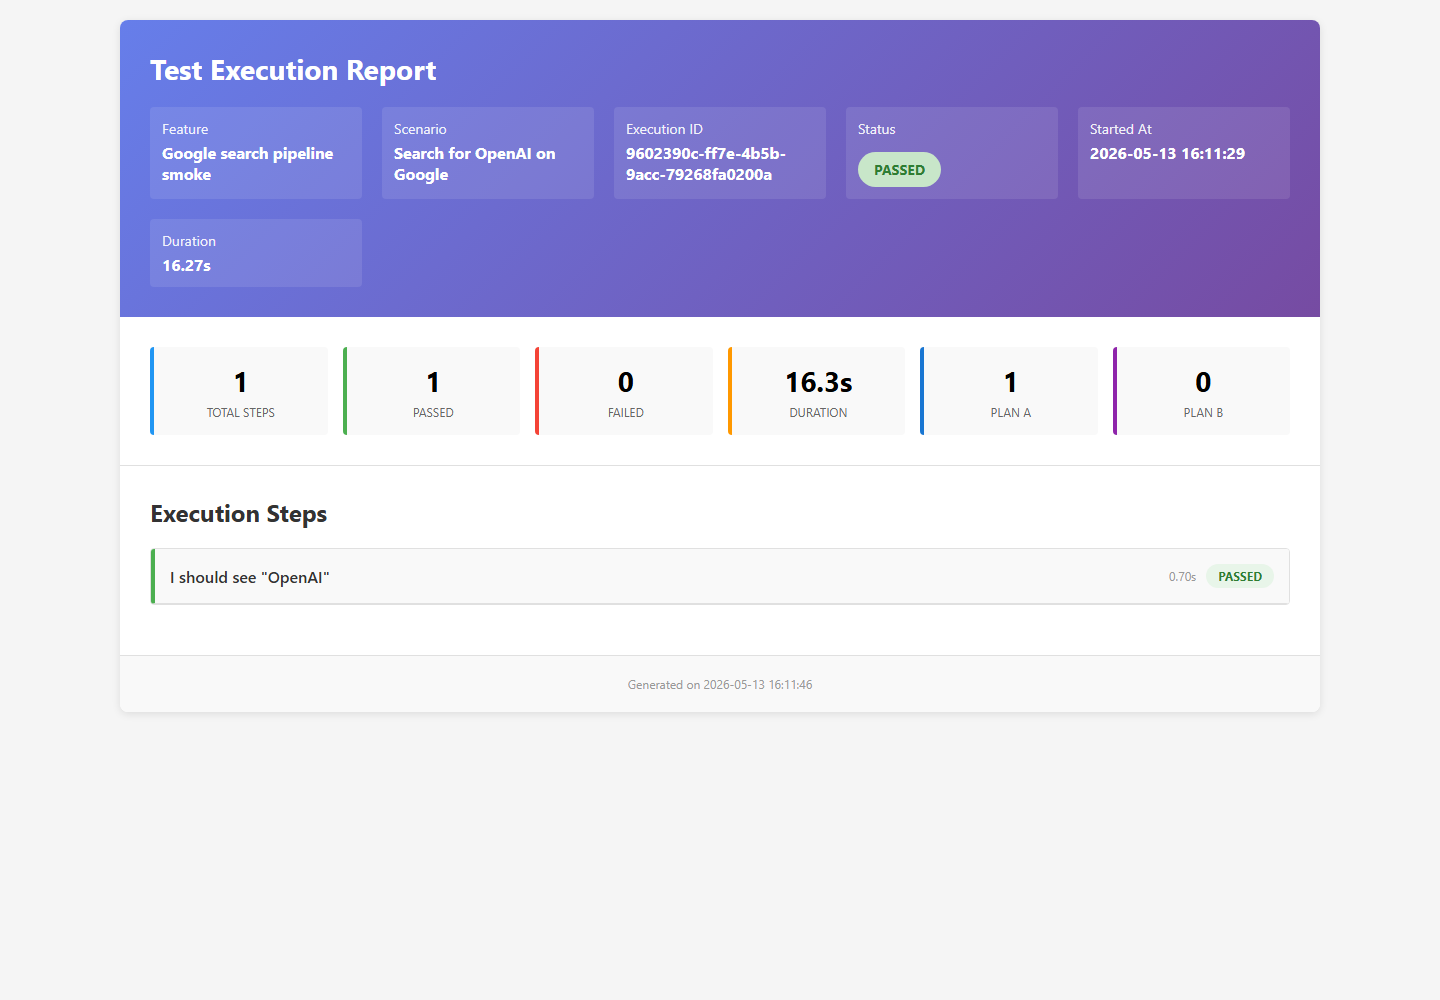
\includegraphics[width=0.95\textwidth]{html_report_example.png}
	\caption{Example of an HTML execution report generated by VisionTest-AI}
	\label{fig:html_report_example}
\end{figure}

\subsection{Screenshot Evidence}
\label{subsec:screenshot_evidence}

Screenshots are captured during execution and linked to the report. They provide visual evidence of what happened during each step. This is especially useful when a test fails, because it allows the user to inspect the actual state of the page.

For example, if a login test fails because an error message is displayed, the screenshot allows the tester to confirm the result visually.


\subsection{Report API Endpoints}
\label{subsec:report_api_endpoints}

The reporting module exposes several API endpoints.

Table~\ref{tab:reporting_endpoints} presents the API endpoints used to list and retrieve generated reports.

\begin{table}[H]
	\centering
	\caption{Reporting API endpoints}
	\label{tab:reporting_endpoints}
	\renewcommand{\arraystretch}{1.35}
	\small
	\begin{tabularx}{\textwidth}{|l|X|}
		\hline
		\rowcolor{gray!20}
		\textbf{Endpoint} & \textbf{Description} \\ \hline
		\texttt{GET /api/ia/reports} & Lists generated reports. \\ \hline
		\texttt{GET /api/ia/reports/\{execution\_id\}} & Retrieves a specific JSON report. \\ \hline
		\texttt{GET /api/ia/reports/\{execution\_id\}?format=html} & Retrieves a specific HTML report. \\ \hline
		\texttt{GET /api/ia/reports/\{execution\_id\}/summary} & Retrieves a compact summary of a report. \\ \hline
	\end{tabularx}
\end{table}

\subsection{Streamlit Report Viewer}
\label{subsec:streamlit_report_viewer}

The Streamlit interface includes a report viewer. This page allows the user to select a generated report, view the HTML version, inspect the JSON file, and check the execution summary.

This feature makes the reporting system more accessible because the user does not need to manually open files from the project directory.

\section{User Interface}
\label{sec:user_interface}

The frontend of the project was implemented using \textbf{Streamlit}~\cite{streamlit_docs}. It provides a simple interface for interacting with the backend services.

\subsection{Scenario Studio}
\label{subsec:scenario_studio}

The Scenario Studio allows the user to write or paste a Gherkin scenario. The scenario can then be parsed, transformed into actions, generated as a Playwright script, or executed directly.

This page represents the main entry point of the system.

Figure~\ref{fig:scenario_studio} shows the Scenario Studio page used to submit and process Gherkin scenarios.

\begin{figure}[H]
	\centering
	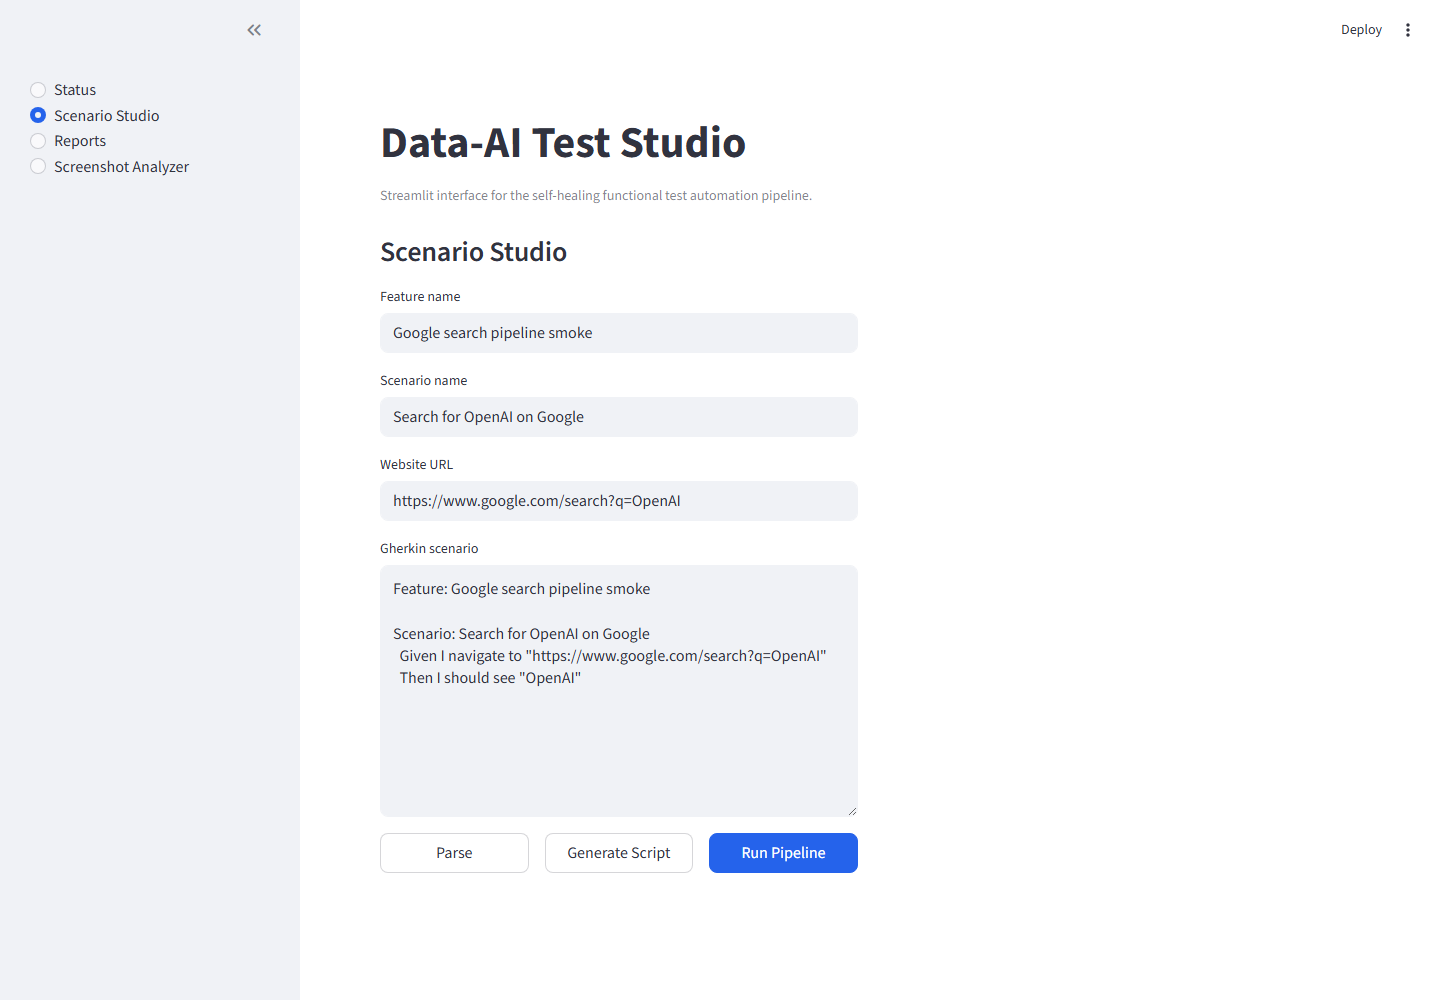
\includegraphics[width=0.95\textwidth]{scenario_studio.png}
	\caption{Scenario Studio interface for submitting Gherkin scenarios}
	\label{fig:scenario_studio}
\end{figure}

\subsection{Script Generation View}
\label{subsec:script_generation_view}

The script generation view displays the Playwright code generated from the submitted Gherkin scenario. This is useful for users who want to inspect, reuse, or manually adapt the generated script.

Figure~\ref{fig:streamlit_generated_script} represents the generated Playwright script as displayed in the Streamlit interface.

\begin{figure}[H]
	\centering
	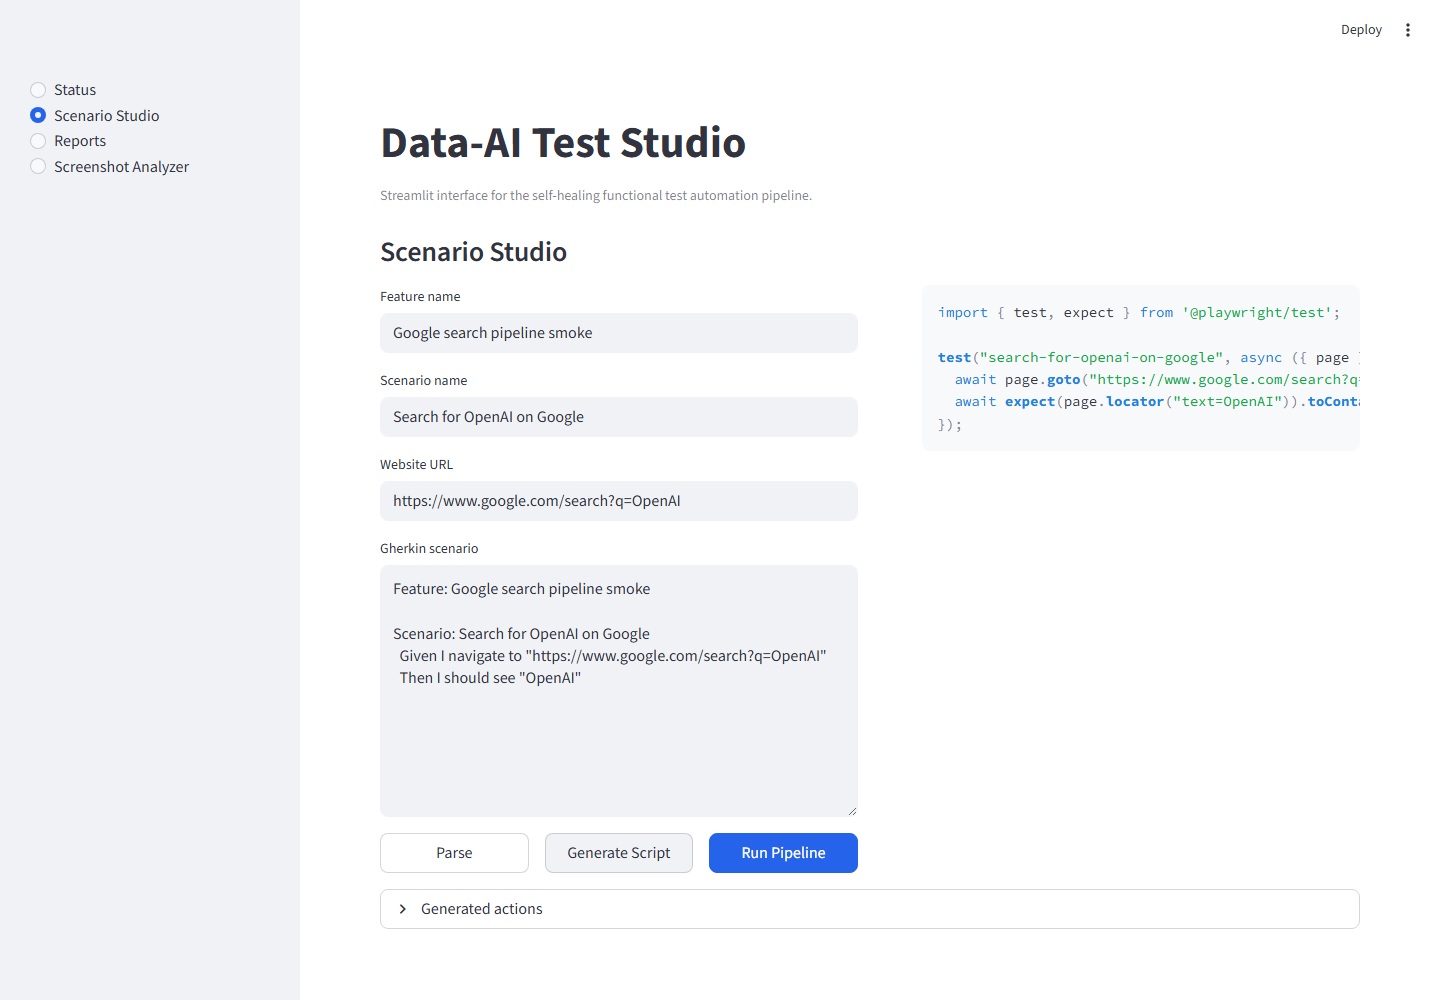
\includegraphics[width=0.95\textwidth]{streamlit_generated_script.png}
	\caption{Generated Playwright script displayed in the Streamlit interface}
	\label{fig:streamlit_generated_script}
\end{figure}

\subsection{Screenshot Analyzer}
\label{subsec:screenshot_analyzer}

The screenshot analyzer allows the user to test the vision module independently. The user can upload a screenshot, activate OCR, define a target text, and view detected elements.

This page was useful during development because it allowed isolated testing of the YOLO/OCR pipeline.


\subsection{Reports Page}
\label{subsec:reports_page}

The reports page allows the user to browse generated reports and inspect previous executions. It provides access to both HTML and JSON versions of each report.

Figure~\ref{fig:reports_page} shows the reports page used to inspect previous executions.

\begin{figure}[H]
	\centering
	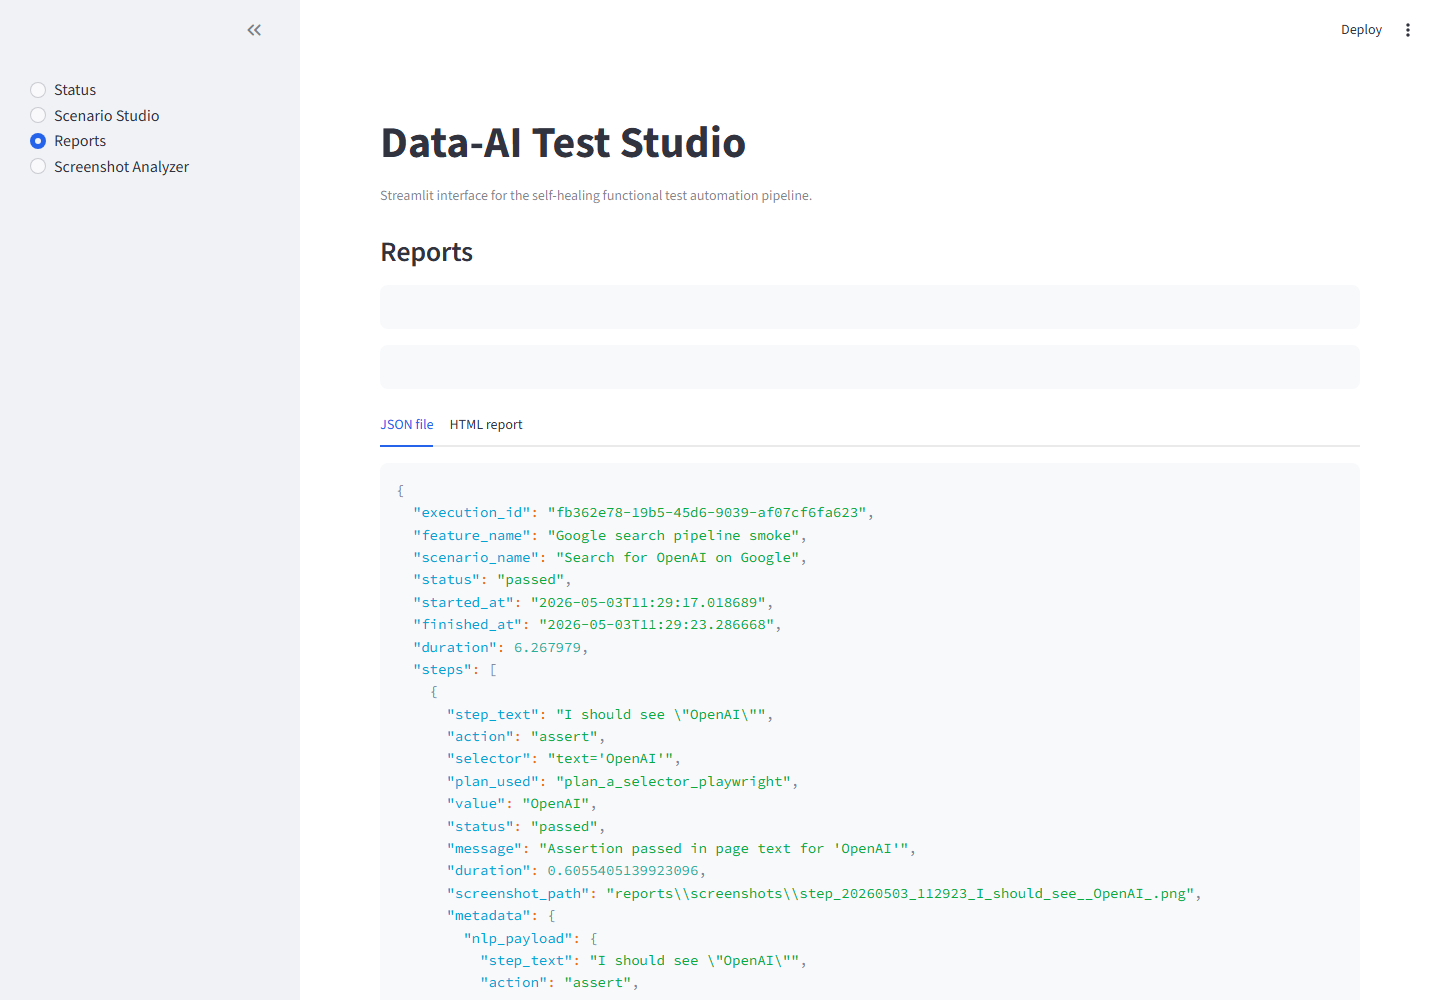
\includegraphics[width=0.95\textwidth]{reports_page.png}
	\caption{Reports page in the Streamlit interface}
	\label{fig:reports_page}
\end{figure}

\section{Deployment Attempts}
\label{sec:deployment_attempts}

Deployment was an important part of the project because the system includes several components: a backend API, browser automation, AI models, OCR dependencies, and a Streamlit frontend.

\subsection{Local Deployment}
\label{subsec:local_deployment}

The first stable deployment was local. The FastAPI backend was launched locally, and the Streamlit interface communicated with it through API calls.

This environment was useful for development and testing because it allowed direct access to logs, screenshots, reports, and model files.

\subsection{Docker Deployment}
\label{subsec:docker_deployment}

\textbf{Docker}~\cite{docker_docs} was considered to make the application easier to run in different environments. Containerization helps package the backend, dependencies, and configuration in a reproducible way.

However, Docker deployment required careful handling of Playwright browsers, OCR dependencies, model files, and report storage. These requirements made deployment more complex than a simple web application.

\subsection{First Streamlit Cloud Attempt}
\label{subsec:streamlit_cloud_attempt}

A first cloud deployment attempt was made using Streamlit Cloud because it is simple and convenient for Python interfaces. However, this approach showed limitations for the full system.

Streamlit Cloud is well suited for lightweight data applications, but \textbf{VisionTest-AI} requires browser automation, AI model loading, OCR, and backend services. Running all these components in the same lightweight environment created resource and configuration problems.

\subsection{Resource Limit Issue}
\label{subsec:resource_limit_issue}

The main issue was resource limitation. Playwright requires browser binaries, YOLO requires model loading, and OCR may require system-level dependencies. These elements can exceed the constraints of a simple Streamlit deployment.

This experience showed that the frontend and backend should not be deployed in the same environment.

\subsection{Final Proposed Architecture: Railway Backend and Streamlit UI}
\label{subsec:final_deployment_architecture}

The final proposed deployment architecture separates the backend from the frontend:

\begin{itemize}
	\item \textbf{FastAPI backend:} Deployed on a platform such as Railway~\cite{railway_docs}.
	\item \textbf{Streamlit frontend:} Deployed separately and configured to call the backend API.
	\item \textbf{Reports and screenshots:} Stored by the backend service.
	\item \textbf{AI models:} Loaded by the backend where more resources are available.
\end{itemize}

This architecture is more realistic because it separates user interaction from heavy processing.

Figure~\ref{fig:deployment_architecture} represents the final proposed deployment architecture. The diagram was created by the author using Mermaid~\cite{mermaid_docs}.

\begin{figure}[H]
	\centering
	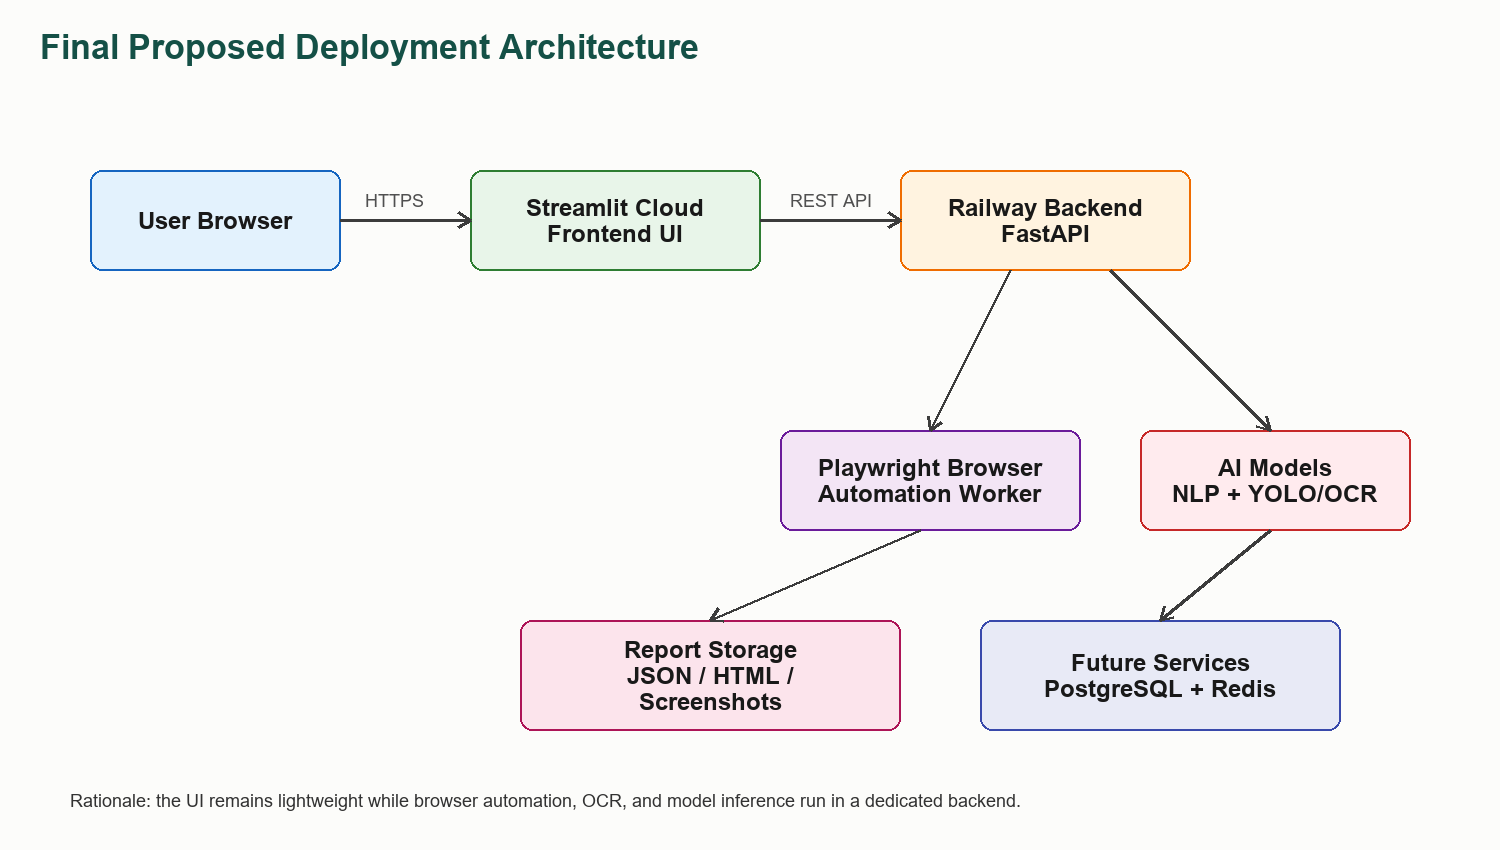
\includegraphics[width=0.95\textwidth]{deployment_architecture.png}
	\caption{Final proposed deployment architecture}
	\label{fig:deployment_architecture}
\end{figure}

\subsection{CI/CD Integration Strategy}
\label{subsec:cicd_strategy}

Although a complete production CI/CD pipeline was not fully deployed during the internship, the project was structured to support this evolution. The objective of the CI/CD strategy is to automate verification before each deployment and reduce the risk of breaking the testing platform itself.

The proposed CI/CD workflow is composed of the following stages:

\begin{enumerate}
	\item \textbf{Source code update:} A developer pushes changes to the project repository.
	\item \textbf{Static verification:} The pipeline checks formatting, dependencies, and basic import errors.
	\item \textbf{Unit and API tests:} Tests are executed for the mapping service, report service, generation service, and API endpoints.
	\item \textbf{Docker build:} The backend image is built with the required Python dependencies, Playwright configuration, OCR tools, and model files.
	\item \textbf{Deployment:} If tests pass, the backend can be deployed to Railway and the Streamlit frontend can be deployed separately.
	\item \textbf{Post-deployment smoke test:} A simple scenario is executed to verify that the API, browser automation, and report generation still work after deployment.
\end{enumerate}

In the current version, the project already contains automated tests and Docker configuration, which represent the foundation of this CI/CD strategy. Future work should connect these steps to a Git-based pipeline in order to automate deployment and validation.

\section{Testing and Validation}
\label{sec:testing_validation}

The system was validated using several types of tests. The objective was to verify individual modules and the complete pipeline.

\subsection{Unit Tests}
\label{subsec:unit_tests}

Unit tests were used to validate isolated services such as the mapping service, report service, generator service, and utility functions.

These tests help ensure that the internal logic remains stable when changes are made.

\subsection{API Tests}
\label{subsec:api_tests}

API tests were used to verify that the main endpoints return correct responses. These tests covered endpoints such as semantic mapping, test generation, segmentation, and reporting.

Example tested endpoints include:

\begin{itemize}
	\item \texttt{/api/ia/semantic-mapping}
	\item \texttt{/api/ia/generate-test}
	\item \texttt{/api/ia/reports}
	\item \texttt{/api/ia/reports/\{execution\_id\}/summary}
\end{itemize}

\subsection{End-to-End Test Scenarios}
\label{subsec:e2e_test_scenarios}

End-to-end scenarios were used to test the complete pipeline. These scenarios started from Gherkin input and ended with generated reports.

The tested workflows included:

\begin{itemize}
	\item Google search scenario.
	\item Facebook login scenario.
	\item Form filling scenario.
	\item Verification of expected text.
\end{itemize}

\subsection{Unseen-Site Benchmark}
\label{subsec:unseen_site_benchmark}

The system was also tested on websites not used during development. This type of testing is important because it checks whether the pipeline can generalize beyond known examples.

The results were mixed. The NLP and mapping modules performed well on explicit steps, while the vision module still depended strongly on the quality of detections and OCR.

\section{Actual Results}
\label{sec:actual_results}

This section presents the main results obtained from the final prototype. The goal is to describe what works, what partially works, and what still needs improvement.

\subsection{Generated JSON Reports}
\label{subsec:generated_json_reports}

The system successfully generated JSON reports after execution. These reports contain structured information about the scenario, steps, screenshots, and execution summary.

Figure~\ref{fig:json_report_example} presents an example of a generated JSON report.

\begin{figure}[H]
	\centering
	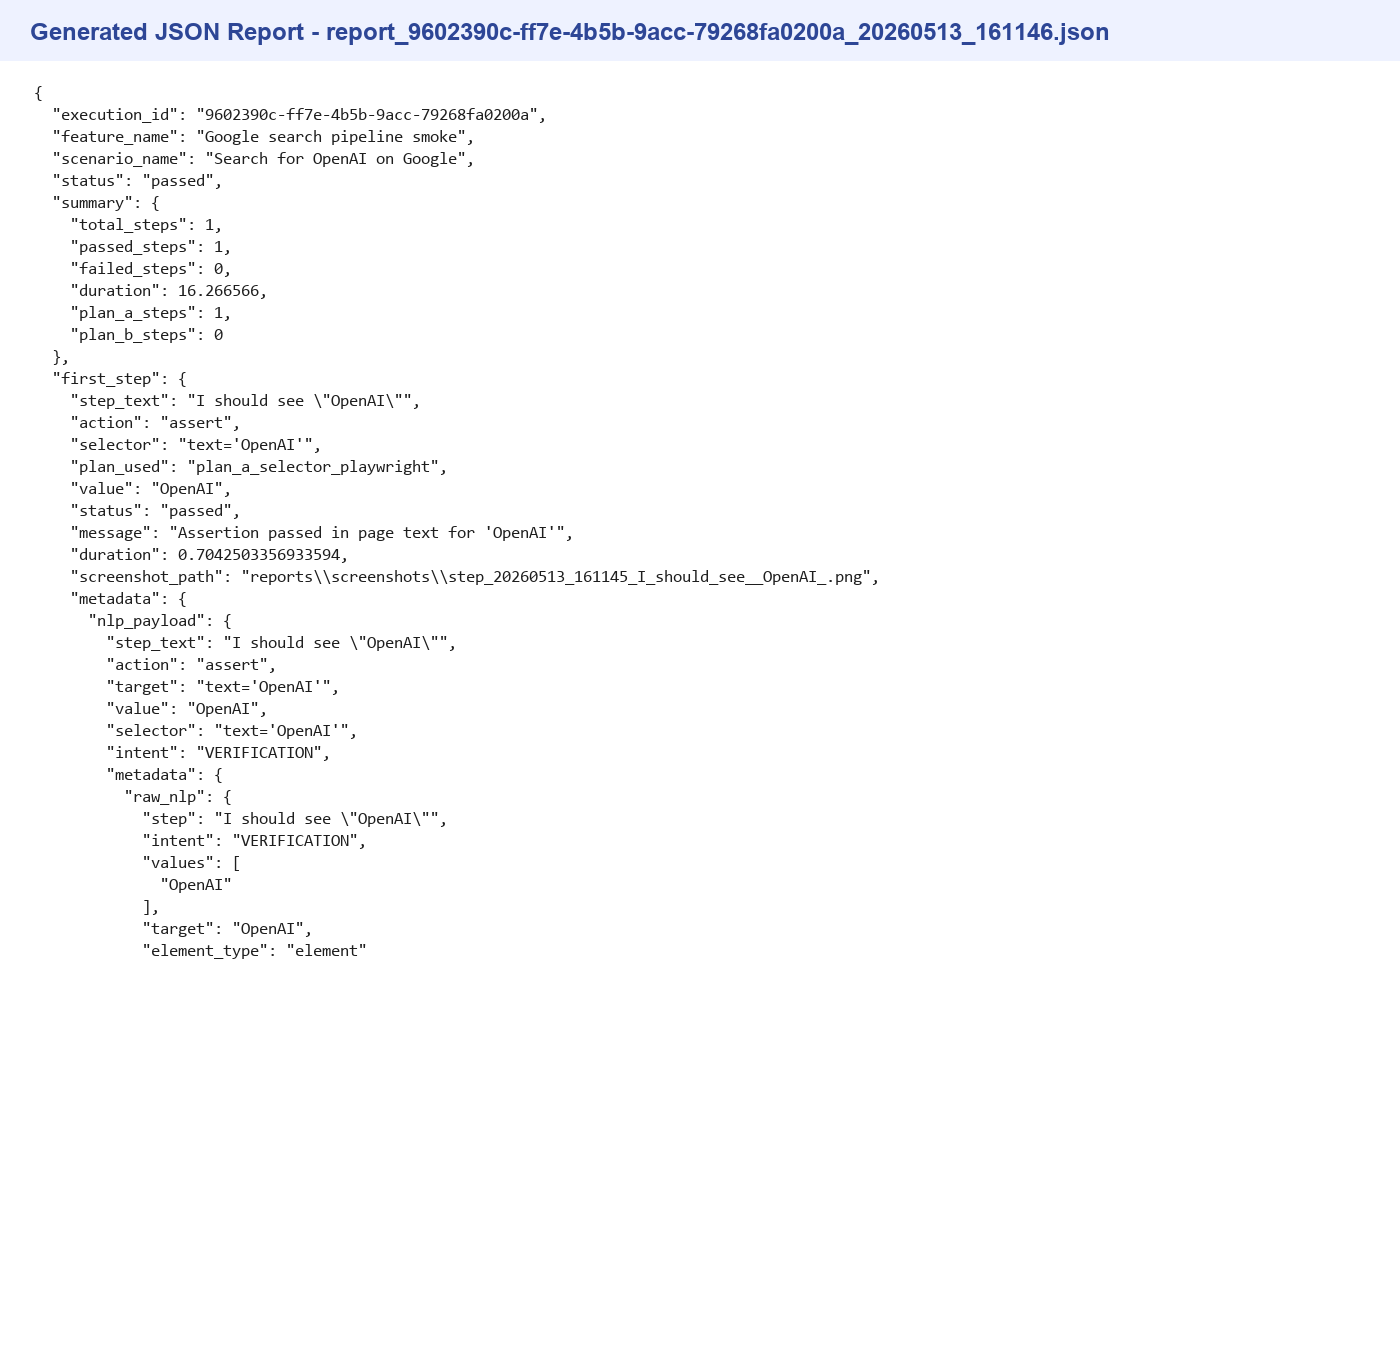
\includegraphics[width=0.95\textwidth]{json_report_example.png}
	\caption{Example of a generated JSON report}
	\label{fig:json_report_example}
\end{figure}

\subsection{Generated HTML Reports}
\label{subsec:generated_html_reports}

The system also generated HTML reports. These reports provide a more readable representation of the execution and are easier to analyze manually.

Figure~\ref{fig:html_report_final} represents the final HTML report generated by the reporting module.

\begin{figure}[H]
	\centering
	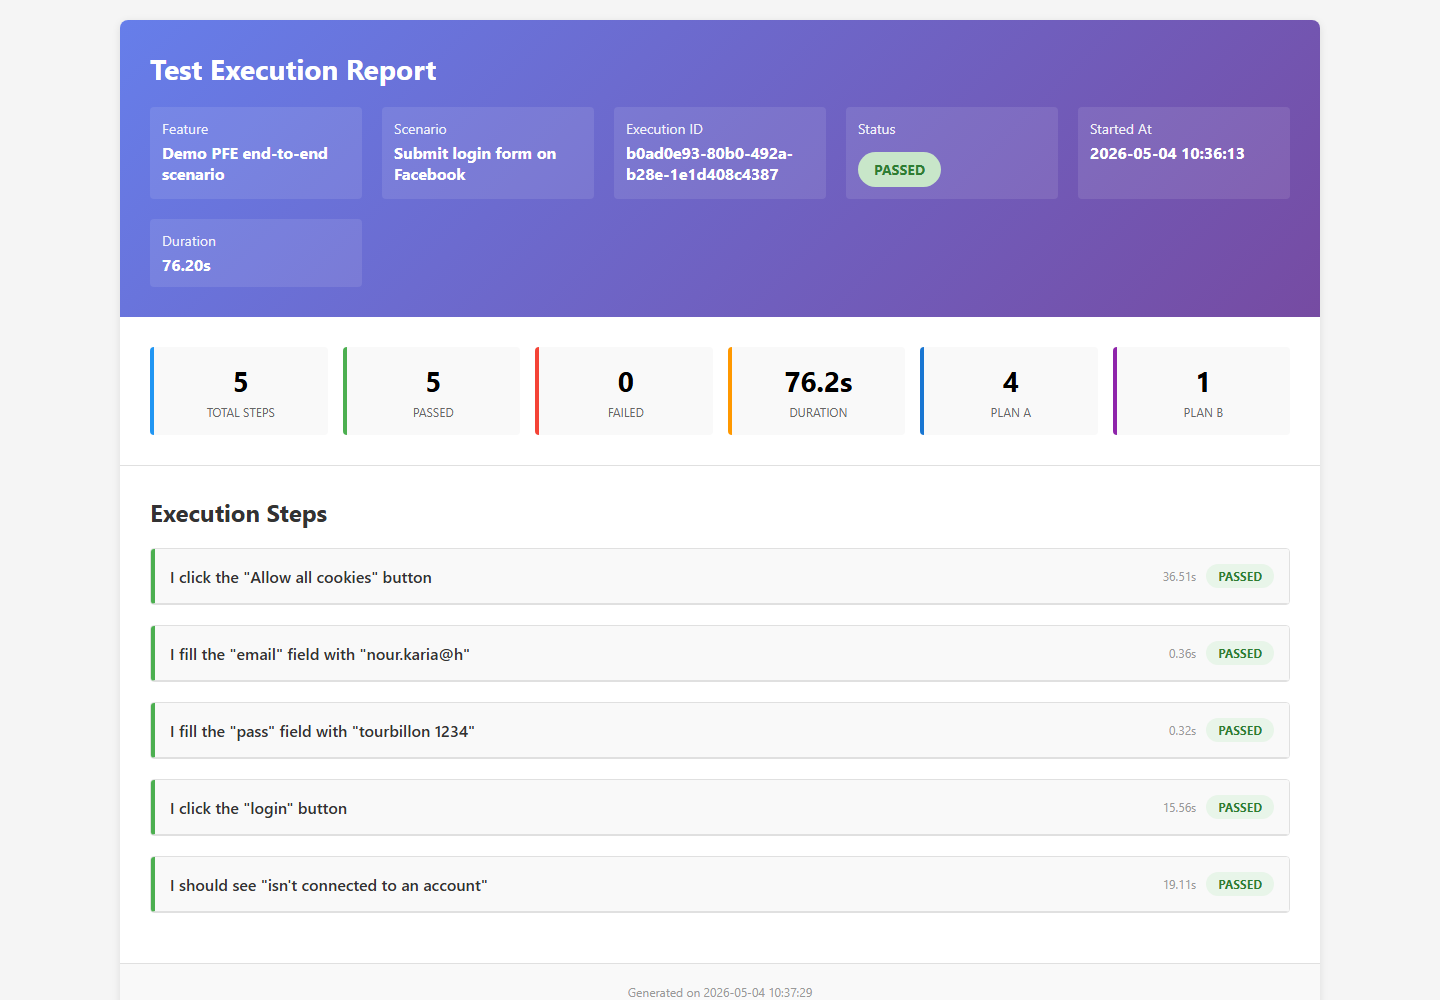
\includegraphics[width=0.95\textwidth]{html_report_final.png}
	\caption{Example of a generated HTML report}
	\label{fig:html_report_final}
\end{figure}

\subsection{Successful Execution Examples}
\label{subsec:successful_execution_examples}

Some scenarios were executed successfully from beginning to end. The most stable cases were scenarios with explicit steps and clear UI targets.

Examples include:

\begin{itemize}
	\item Navigating to a target page.
	\item Filling a visible input field.
	\item Clicking a clearly identified button.
	\item Verifying that expected text appears on the page.
\end{itemize}

\subsection{Failed Execution Examples}
\label{subsec:failed_execution_examples}

Some scenarios failed due to selector issues, page changes, popups, OCR errors, or ambiguous targets. These failures were useful because they helped identify the current limits of the system.

Table~\ref{tab:failed_execution_cases} lists representative failed execution cases and possible improvements.

\begin{table}[H]
	\centering
	\caption{Examples of failed execution cases}
	\label{tab:failed_execution_cases}
	\renewcommand{\arraystretch}{1.35}
	\small
	\begin{tabularx}{\textwidth}{|X|X|X|}
		\hline
		\rowcolor{gray!20}
		\textbf{Failure Case} & \textbf{Cause} & \textbf{Possible Improvement} \\ \hline
		Button not clicked & Selector failed and visual detection was not precise enough. & Improve YOLO dataset and candidate ranking. \\ \hline
		Wrong element selected & Several visual candidates were similar. & Combine OCR, DOM context, and semantic scoring. \\ \hline
		OCR text incorrect & Text was small or low contrast. & Improve preprocessing and OCR configuration. \\ \hline
		Cloud execution issue & Deployment environment lacked required resources. & Separate backend and frontend deployment. \\ \hline
	\end{tabularx}
\end{table}

\subsection{Plan A vs Plan B Usage}
\label{subsec:plan_a_plan_b_usage}

The execution strategy is divided into Plan A and Plan B. Plan A uses Playwright selectors, while Plan B uses visual fallback.

In the current version, Plan A remains the most reliable strategy when selectors are valid. Plan B is useful in some cases, but its success depends on YOLO detection quality, OCR readability, and target ranking.

Table~\ref{tab:plan_a_plan_b} compares the two execution strategies used by the system.

\begin{table}[H]
	\centering
	\caption{Comparison between Plan A and Plan B}
	\label{tab:plan_a_plan_b}
	\renewcommand{\arraystretch}{1.35}
	\small
	\begin{tabularx}{\textwidth}{|l|X|X|}
		\hline
		\rowcolor{gray!20}
		\textbf{Strategy} & \textbf{Strengths} & \textbf{Limitations} \\ \hline
		Plan A: Playwright selectors & Fast, precise, reliable when DOM is stable. & Breaks when selectors change or elements are hard to locate. \\ \hline
		Plan B: YOLO/OCR fallback & Can recover when the element is visible but selectors fail. & Depends on model accuracy, OCR quality, and ranking logic. \\ \hline
	\end{tabularx}
\end{table}

\subsection{Performance Observations}
\label{subsec:performance_observations}

The NLP and semantic mapping modules are lightweight and respond quickly for simple scenarios. Playwright execution time depends mainly on page loading, network speed, and browser behavior.

The vision module is more expensive because it requires screenshot processing, YOLO inference, and OCR. For this reason, it is only activated when needed, rather than being used for every action.

This design keeps the normal execution path efficient while still allowing fallback when necessary.

\section{Limitations}
\label{sec:chapter5_limitations}

The final prototype achieved the main objective of connecting Gherkin understanding, test generation, execution, vision fallback, and reporting. However, several limitations remain.

\subsection{Model Accuracy Limitations}
\label{subsec:model_accuracy_limitations}

The YOLO model still requires improvement. Some detections are inaccurate, especially for small elements, dense interfaces, or visually similar components. The dataset must be expanded and cleaned further to improve model generalization.

\subsection{OCR Limitations}
\label{subsec:ocr_limitations}

OCR performance depends on image quality, font size, contrast, and page layout. In some cases, OCR extracted incorrect or incomplete text, which affected target matching.

\subsection{Deployment Resource Limitations}
\label{subsec:deployment_resource_limitations}

The deployment phase showed that the system requires more resources than a simple Streamlit application. Browser automation, OCR, and AI model inference should be handled by a dedicated backend service.

\subsection{Lack of PostgreSQL and Redis Integration}
\label{subsec:postgres_redis_limitations}

The current version stores reports as local JSON and HTML files. This is sufficient for a prototype, but not ideal for a production system.

A future version should use:

\begin{itemize}
	\item \textbf{PostgreSQL} for persistent storage of projects, executions, users, and reports.
	\item \textbf{Redis} for caching, queues, and background execution management.
\end{itemize}

\section{Perspectives}
\label{sec:perspectives}

Several improvements can be added in future versions of \textbf{VisionTest-AI}.

\subsection{Improve NLP Multilingual Support}
\label{subsec:improve_multilingual_support}

The current NLP module mainly supports English scenarios. Future work should add support for French and mixed-language Gherkin scenarios.

\subsection{Expand the Annotated Dataset}
\label{subsec:expand_dataset}

The vision dataset should be expanded with more websites, component libraries, screen sizes, themes, and UI styles. This would improve YOLO detection quality and reduce false positives.

\subsection{Add PostgreSQL and Redis}
\label{subsec:add_postgres_redis}

A production version should include database and queue services. PostgreSQL can store reports and project history, while Redis can manage background tasks and improve performance.

\subsection{Add Authentication and Project History}
\label{subsec:add_auth_project_history}

Authentication would allow multiple users to manage their own projects, scenarios, and reports. Project history would make it possible to compare executions over time.

\subsection{Improve Cloud Deployment}
\label{subsec:improve_cloud_deployment}

The final deployment architecture should separate the frontend, backend, browser execution, model inference, and report storage. This would make the system more stable and scalable.

\section{Conclusion}
\label{sec:ch5_conclusion}

This chapter presented the final integration of \textbf{VisionTest-AI}. It showed how the different modules are connected to form a complete pipeline, starting from a Gherkin scenario and ending with JSON and HTML execution reports.

The backend implementation was organized around FastAPI routers and services. The Streamlit interface provided access to scenario submission, script generation, screenshot analysis, and report viewing. The reporting system made it possible to store and inspect execution evidence.

The deployment attempts showed that the system is more complex than a simple web application because it includes browser automation, AI models, OCR, screenshots, and reports. This led to the final proposed architecture based on a separated backend and frontend.

The final results confirm that the prototype can parse scenarios, generate Playwright scripts, execute tests, produce reports, and activate visual fallback in some cases. However, the project still has limitations related to YOLO accuracy, OCR reliability, deployment resources, and missing production features such as PostgreSQL, Redis, authentication, and project history.

Overall, \textbf{VisionTest-AI} demonstrates the feasibility of an intelligent functional testing agent that combines semantic understanding, browser automation, visual perception, and reporting. The system provides a solid foundation for future improvements and industrialization.

\chapter*{General Conclusion and Perspectives}
\addcontentsline{toc}{chapter}{General Conclusion and Perspectives}
\label{chap:general_conclusion}

This graduation project focused on the design and implementation of \textbf{VisionTest-AI}, an intelligent functional testing agent that combines natural language understanding, browser automation, visual perception, and automatic reporting. The main objective was to reduce the fragility of traditional automated tests by allowing the system to understand Gherkin scenarios, generate executable actions, execute them with Playwright, and use visual fallback mechanisms when classical selectors fail.

Throughout the project, we built a complete prototype composed of several modules. The NLP module parses Gherkin scenarios, classifies intents, extracts entities, and prepares structured action payloads. The semantic mapping module transforms these actions into Playwright-compatible commands and selector candidates. The execution service runs the test steps in a browser, while the vision module uses YOLOv8n and OCR to detect UI elements from screenshots when selector-based execution is not sufficient. Finally, the reporting service generates JSON and HTML reports containing execution details, screenshots, errors, and summary metrics.

One of the main achievements of this work is the integration of several technologies into a single functional pipeline. The project does not only generate scripts or analyze screenshots separately; it connects these components into a complete workflow, starting from a business-readable Gherkin scenario and ending with an execution report. This demonstrates the feasibility of an intelligent testing assistant that can support QA engineers in writing, executing, and analyzing functional tests.

The project also highlighted several technical challenges. Preparing a reliable UI detection dataset was more difficult than expected. Ready-made datasets were not diverse enough, manual annotation was time-consuming, and automatic labeling required several corrections before becoming usable. The final DOM-assisted labeling approach helped improve the quality of annotations, but the YOLO model still needs more training data and refinement. Deployment was another challenge, especially because the system requires browser automation, OCR, AI models, and report storage, which makes it heavier than a simple Streamlit application.

The obtained results are encouraging. The NLP and semantic mapping modules successfully handled explicit functional steps such as navigation, input, click, and verification. The system was able to generate Playwright scripts, execute scenarios, capture screenshots, and produce structured JSON and HTML reports. The visual fallback mechanism also showed its value in some cases, especially when the target element was visible but the selector-based strategy failed.

However, the current version remains a prototype and has several limitations. The vision module is not yet fully reliable on all interfaces, OCR can fail on small or low-contrast text, and some complex interactions such as drag-and-drop, file upload, or advanced dynamic components are not fully supported. The system also does not yet include production features such as authentication, project history, PostgreSQL storage, Redis queues, or advanced cloud orchestration.

Several perspectives can be considered for future work. The NLP module can be improved by adding multilingual support, especially for French and mixed-language Gherkin scenarios. The vision dataset can be expanded with more annotated examples from different websites, themes, and component libraries. The execution engine can be enhanced with better ranking logic, stronger self-healing strategies, and support for more complex user actions. On the platform side, adding PostgreSQL, Redis, authentication, and project management features would make the system closer to an industrial solution.

In conclusion, \textbf{VisionTest-AI} provides a solid foundation for an AI-assisted functional testing platform. It shows that combining semantic understanding with visual perception can make test automation more flexible and more resilient. Although further improvements are still required, the project successfully demonstrates how AI techniques can be applied to modern QA workflows in a practical and extensible way.

\bibliographystyle{plain}
\bibliography{references/allbiblio}

%\include{chapters/annexe}

\end{document}
